% Great thanks for Cezary Sałbut (this latex file is mainly based on his work)

\documentclass[a4paper,12pt,fleqn]{article}


\usepackage[utf8]{inputenc} 
\usepackage{polski}
\usepackage[polish]{babel}
\usepackage[pdftex]{color,graphicx}
\usepackage{subfig}
\usepackage{indentfirst}
\usepackage{booktabs}
\usepackage{tabularx}
\usepackage{multirow}
\usepackage{pdflscape}
\usepackage{array}
\usepackage{amsmath}
\usepackage{appendix}
\usepackage{hyperref}
\hypersetup{
    colorlinks,%
    citecolor=black,%
    filecolor=black,%
    linkcolor=black,%
    urlcolor=blue
}

\usepackage{listings}
\lstset{
	numbers=left, 
	stepnumber=1, 
	basicstyle={\footnotesize \ttfamily},
	language=C, 
	captionpos=b,
	xleftmargin=6mm,
	aboveskip=\medskipamount,
	belowskip=\bigskipamount,
	tabsize=4
}

\usepackage{title-page}

\usepackage[top=28mm, bottom=30mm, left=21mm, right=21mm]{geometry}

\linespread{1.5}		%interlinia

\usepackage{boxedminipage} 
%% change the below lengths to suit your needs: 
\setlength{\fboxrule}{1pt} 
\setlength{\fboxsep}{5pt}



\renewcommand{\appendixtocname}{Dodatki}
\renewcommand{\appendixpagename}{Dodatki}


\widowpenalty=10000
\clubpenalty=10000


\newcommand{\autor}{Jan Kurdel}
\newcommand{\tytulpl}{Identyfikacja nieliniowych obiektów dynamicznych metodą uogólnionej regresji postępującej z ortogonalizacją}
\newcommand{\tytulen}{Identification of nonlinear dynamical objects based on Generalized Orthogonal Forward Regression}
\newcommand{\uczelnia}{POLITECHNIKA WARSZAWSKA}
\newcommand{\wydzial}{Wydział Elektroniki i Technik Informacyjnych}
\newcommand{\instytut}{Instytut Systemów Elektronicznych}
\newcommand{\promotor}{dr inż. Stanisława Jankowskiego}
\newcommand{\praca}{Praca inżynierska}
\newcommand{\miejscerok}{Warszawa, 2012}
\newcommand{\indeks}{214460}

\title{\tytulpl}
\author{\autor}

\begin{document}

\renewcommand{\tablename}{Tabela}

\pagestyle{empty}
\stronatytulowa

\newpage
\setcounter{page}{1}

\newpage
\textbf{\tytulpl} \vspace*{0.2cm} \\
Praca opisuje identyfikację obiektów dynamicznych metodą uogólnionej regresji postępującej z ortogonalizacją. Identyfikacja została przeprowadzona na przykładzie nieliniowego obiektu dynamicznego opisanego równaniem Van der Pola. Jakość modelu została następnie oceniona na podstawie błędu średniokwadratowego predykcji na 100 kroków w przód. Model był testowany dla 440 różnych warunków początkowych. Zastosowana metoda pozwoliła poprawnie odwzorować obiekt dynamiczny dla zdecydowanej większości warunków początkowych.

\vspace*{2cm}
\textbf{\tytulen} \vspace*{0.2cm} \\
The object of the thesis is identification of nonlinear dynamical objects based on Generalized Orthogonal Forward Regression method. Identification was based on nonlinear dynamical object described by Van der Pol differential equation. Quality of model was evaluted on basis of Mean Squared Error of 100 step prediction. Model was tested for set of 440 different initial conditions. Applied method well model dynamical object for the vast majority of initinal conditions.

\newpage
\tableofcontents

\newpage
\pagestyle{plain}

\section{Cel pracy}
	W dzisiejszych czasach częstą koniecznością jest tworzenie modeli matematycznych rzeczywistych obiektów. Model matematyczny obiektu opisuje związek między sygnałem podawanym na wejście (sterowaniem) oraz sygnałem wyjściowym. Modelowanie takie wykorzystuje się pracując nad silnikami, robotami przemysłowymi, klimatyzacją, systemami hamulcowymi\cite{Isermann}. Oprócz szerokiego spektrum dziedzin, w których ma zastosowanie tworzenie modeli, istnieje szereg różnych metod ich tworzenia na postawie danych doświadczalnych, czyli metod identyfikacji obiektów.
	
	Wśród metod identyfikacji można spotkać się metodą charakterystyk czasowych, w której badane są stany przejściowe po podaniu na wejście obiektu określonego wymuszenia, np. odpowiedzi na skok jednostkowy. Inna metodą jest metoda charakterystyk częstotliwościowych gdzie na wejście podaje się sygnał sinusoidalny o zadanej amplitudzie i częstotliwości a badany jest sygnał wyjściowy - jego amplituda oraz przesunięcie fazowe względem sygnału wejściowego\cite{Czemplik}.
	
	W pracy zdecydowano się na inną metodę identyfikacji dynamiki obiektu - wykorzystano w tym celu sieć neuronową. Można spotkać się z wieloma przykładami zastosowania sieci neuronowych w zadaniu identyfikacji dynamiki jednak struktura oraz algorytmy trenowania takiej sieci  mogą znacznie się różnić. W pracy zostanie przedstawiona metoda uogólnionej regresji postępującej z ortogonalizacją (Generalized Orthogonal Forward Regressoin - GOFR) oraz jej wykorzystanie do identyfikacji nieliniowego obiektu dynamicznego opisanego równaniem różniczkowym Van der Pola. Następnie zostanie dokonana ocena jakości modelowania z wykorzystaniem zaproponowanego rozwiązania. Równanie Van der Pola ma zastosowanie między innymi w dziedzinie układów elektronicznych\cite{Palczewski}. Należy zaznaczyć, że zaproponowany algorytm może mieć zastosowanie również do obiektów opisanych innymi równaniami różniczkowymi.  

\newpage
\section{Dynamika obiektów}
Układ dynamiczny to matematyczny model, który opisuje ewolucję realnego zjawiska. Model taki pozwala na analizę reakcji badanego obiektu na pojawiające się zmiany.
Układ dynamiczny z czasem ciągłym jest opisywany układem równań ruchu w postaci ogólnej\cite{Kosinski}
\begin{equation}
	\frac{dx}{dt} = F(x,r), \quad x \in R
\end{equation}

gdzie: \\
$F$ - odwzorowanie $F:U \rightarrow R^n$,
$r$ - zbiór parametrów kontrolnych układu,
$U$ – podzbiór $R^n$ określający przestrzeń fazową układu.

Przestrzeń fazowa jest przestrzenią wszystkich możliwych stanów w jakich może znajdować się badany układ. Każdy stan układu jest pojedynczym punktem tej przestrzeni. Konkretne rozwiązanie układu równań ruchu $\phi_i(t_0,r)$ - dla danych wartości parametrów $r$ i warunków początkowych zwane jest orbitą (trajektorią). Jeśli odwzorowanie $F$ jest odwzorowaniem liniowym to układ dynamiczny jest układem liniowym, natomiast jeśli $F$ jest odwzorowaniem nieliniowym to układ dynamiczny nazywamy układem nieliniowym.

Uniwersalnym sposobem opisu dynamiki obiektów z czasem ciągłym są równania różniczkowe. Dla opisu dynamiki obiektów z czasem dyskretnym odpowiednio stosowane są równania różnicowe\cite{Gutenbaum}.
\subsection{Równania różniczkowe zwyczajne}

Równaniem różniczkowym zwyczajnym nazywamy równanie zawierające zmienną niezależną $x$, nieznaną funkcję $y$, oraz jej pochodne $y', y'', \hdots, y^{(n)}$ \cite{BCh_2001}
\begin{equation}
	\label{wzor:rownanie_roz_N_stopnia}
	F(x,y,y',\hdots,y^{(n)}) = 0
\end{equation}
gdzie $F:R^{n+2} \rightarrow R$

Warunek początkowy (Cauchy'ego) dla równania \ref{wzor:rownanie_roz_N_stopnia} określony jest poprzez: 
\begin{equation}
\begin{array}{c}
y(x_0)       =  y_0,     \\
y'(x_0)      =  y_1,     \\
\vdots			   	     \\
y^{n-1}(x_0) = y_{n-1}
\end{array}
\end{equation}
gdzie $y_0, y_1, \hdots, y_{n-1}$ są zadanymi liczbami.

Stopień pochodnej w równaniu \ref{wzor:rownanie_roz_N_stopnia} decyduje o rzędzie równania różniczkowego. Równanie różniczkowe pierwszego rzędu wyraża się zatem wzorem:
\begin{equation}
	\label{wzor:rownanie_roz_I_stopnia}
	y' = f(x,y)
\end{equation}

Rozwiązanie równania \ref{wzor:rownanie_roz_I_stopnia} w sposób numeryczny może zostać rozwiązane z wykorzystaniem wielu sposobów. Można wyróżnić podział na metody jednokrokowe, które wymagają jedynie informacji z poprzedniego kroku (zatem warunek początkowy jest wystarczający do obliczenia równania różniczkowego dla kolejnego punktu) oraz metody wielokrokowe, w których rozwiązanie jest dokonowywane z wykorzystaniem znajomości kilku poprzednich kroków. Wśród metod jednokrokowych znajdują się m.in. metody Eulera oraz Rungego-Kutty.

\subsection{Metody rozwiązywania równań różniczkowych}

\subsection*{Metoda Eulera}
Metoda Eulera jest najprostszą metodą numeryczną rozwiązywania równań różniczkowych. Mając dane równanie \ref{wzor:rownanie_roz_I_stopnia} oraz warunek początkowy postaci:
\begin{equation}
	y(x_0) = y_0	
\end{equation}
poszukujemy rozwiązania dla kolejnego momentu $x_1 = x_0 + h$ gdzie $h$ jest krokiem metody. W tym celu możemy skorzystać z rozwinięcia szeregu Taylora w pobliżu punktu początkowego $x_0$:
\begin{equation}
	y(x_0 + h) = y(x_0) + hy'(x_0) + \frac{h^2}{2!}y''(x_0) + \hdots
\end{equation}
Korzystając tylko z dwóch pierwszych elementów szeregu Taylora otrzymamy:
\begin{equation}
	y(x_0 + h) = y(x_0) + hy'(x_0) = y(x_0) + hf(x_0,y_0)
\end{equation}
Powtarzając tę czynność wielokrotnie otrzymamy wzór:
\begin{equation}
	y_{n+1} = y_{n} + hf(x_n,y_n)
\end{equation}
określany jawną metodą Eulera.

\subsection*{Metoda Rungego-Kutty}
Kolejną metodą numerycznego rozwiązywania równań różniczkowych jest metoda \mbox{Rungego-Kutty}, która jest metodą wieloetapową. W każdym kroku konieczne jest obliczenie wartości funkcji $f$ dla różnych argumentów. Wśród metod Runge-Kutty można wyróżnić różne warianty tej metody w zależności od rzędu metody. Najprostszą z nich jest metoda Runge-Kutty rzędu II. Przyjmuje ona postać:
\begin{equation}
	y_{i+1} = y_i + \frac{h}{2}(k_1 + k_2)
\end{equation}
gdzie
$$\begin{array}{c}
	k_1 = f(t_i,y_i) \\
	k_2 = f(t_i + h, y_i + hk_1)
\end{array}$$

Najbardziej popularną jest metoda rzędu IV, która przyjmuje postać:
\begin{equation}
	y_{i+1} = y_i + \frac{h}{6}(k_1 + 2k_2 + 2k_3 + k_4)
\end{equation}
gdzie
$$\begin{array}{c}
	k_1 = f(t_i,y_i) \\
	k_2 = f(t_i + \frac{h}{2}, y_i + \frac{h}{2}k_1) \\
	k_3 = f(t_i + \frac{h}{2}, y_i + \frac{h}{2}k_2) \\
	k_4 = f(t_i + h,y_i + hk_3) \\
\end{array}$$

\subsection*{Równania różniczkowe zwyczajne wyższych rzędów}
Równanie różniczkowe wyższych rzędów może zostać sprowadzone do układu równań różniczkowych rzędu pierwszego \cite{AK_RBG2002}. Mając dane równanie różniczkowego n-tego rzędu:
$$y^{(n)}(t) = f(t,y(t),y'(t),\hdots,y^{(n-1)}(t)), \qquad a \leq t \leq b$$
z warunkiem początkowym w postaci:

$$\begin{array}{c}
y(a)       = \alpha_0,    \\
y'(a)      = \alpha_1,    \\
\vdots					  \\
y^{n-1}(a) = \alpha_{n-1} \\
\end{array}$$

oraz wprowadzając nowe zmienne:
$$y_1(t) = y(t), y_2(t) = y'(t), \hdots, y_n(t) = y^{(n-1)}(t)$$

otrzymujemy układ równań różniczkowych pierwszego rzędu postaci:
$$\begin{array}{l}
y'_1       = y_2   \\
y'_2       = y_3   \\
\vdots			   \\
y'_{n-1} = y_n     \\
y'_n = f(t,y_1,y_2,\hdots,y_n)
\end{array}$$

z warunkami początkowymi postaci:
$$y_1(a) = \alpha_0, y_2(a) = \alpha_1, \hdots, y_n(a) = \alpha_{n-1}$$

Dzięki takiemu zabiegowi możliwe jest rozwiązanie równania różniczkowego wyższego rzędu metodami służącymi do rozwiązywania równań różniczkowych rzędu pierwszego.

Należy zaznaczyć, że wymienione metody rozwiązywania równań różniczkowych mogą mieć zastosowanie jedynie w przypadku znajomości postaci równania różniczkowego.
 
\newpage
\section{Sieci neuronowe} 

Sieci neuronowe w dzisiejszych czasach mają bardzo szerokie zastosowanie. Wykorzystywane są m. in do zadań klasyfikacji, aproksymacji, predykcji, sterowania w wielu różnych dziedzinach życia. Sama definicja czym jest sieć neuronowa nie została sprecyzowana ale sieci neuronowe można określić jako adaptacyjne metody tworzenia modeli nieliniowych na podstawie danych eksperymentalnych bądź też formalne modele statystyczne zbudowane na podstawie danych eksperymentalnych\cite{Jankowski}.
 
\subsection{Struktura sieci neuronowych}
Podstawą budowy sieci neuronowych są neurony. Budowa pojedynczego neuronu jest przedstawiona na rysunku \ref{fig:neuron}. Neuron taki sumuje sygnał podany na jego wejścia $x_i$ z odpowiednimi wagami $w_i$, dając na wyjście wynik $y$ sumy przeprowadzonej przez funkcję aktywacji $f(x)$.
\begin{figure}[ht!]
	\centering
	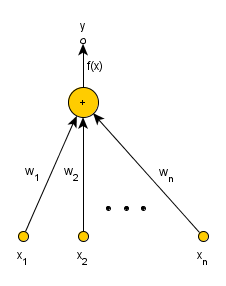
\includegraphics[scale=0.8]{images/single_neuron.png}
	\caption{Budowa pojedynczego neuronu}
	\label{fig:neuron}
\end{figure}

Sieć neuronową budują grupy połączonych ze sobą neuronów. Uproszczoną strukturę sieci wielowarstwowej przedstawia rysunek \ref{fig:multilayer}. Pierwsza warstwa nosi nazwę warstwy wejściowej (\textit{Input}), ostatnia warstwa sieci nosi nazwę warstwy wyjściowej (\textit{Output}). Wszystkie pozostałe warstwy noszą nazwę warstw ukrytych (\textit{Hidden}).

\begin{figure}
	\centering
	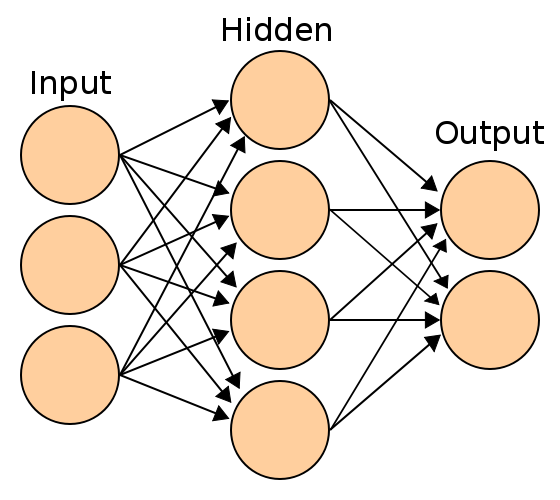
\includegraphics[width=0.5\textwidth]{images/560px-Artificial_neural_network.png}
	\caption{Schemat budowy wielowarstwowej sieci neuronowej \\
	\footnotesize{\textit{źródło:} http://commons.wikimedia.org/wiki/File:Artificial\_neural\_network.svg} }
	\label{fig:multilayer}
\end{figure}

\subsubsection*{Perceptron wielowarstwowy}
Często wykorzystywany typem sieci jest perceptron wielowarstwowy, którą stanowi jednokierunkowa wielowarstwowa sieć o neuronach typu sigmoidalnego (z sigmoidalną funkcją aktywacji)\cite{Osowski}. Funkcja aktywacji często przyjmuje postać $f(x) = \frac{1}{1 + exp(-\beta x)}$ określanej mianem funkcji unipolarnej, bądź też $f(x) = tgh(\beta x)$ określanej mianej funkcji bipolarnej.
 
\subsubsection*{Sieć RBF}
Sieć RBF (Radial Basis Function) jest sztuczną siecią neuronową o radialnych funkcjach bazowych. Sieć ta ma szerokie zastosowanie i jest wykorzystywana do szeregu problemów m.in: modelowania 3D, rozpoznawania mowy, identyfikacji systemów, modelowania parametrów urządzeń elektronicznych\cite{Bors}. Sieć taka składa się zazwyczaj z jednej warstwy ukrytej, gdzie funkcja aktywacji jest radialną funkcją bazową oraz warstwy wyjściowej w postaci neuronu liniowego. Radialna funkcja bazowa jest określona w sposób następujący\cite{Bartkowiak}
\begin{equation}
	G(x,c) = G(r(x,c))
\end{equation}
gdzie $r(x,c)$ jest odległością między punktami $r$ i $c$ a centrum $c$ jest ustalone i pełni rolę parametru funkcji. Jedną z bardziej popularnych radialnych funkcji bazowych jest funkcja Gaussa:
\begin{equation}
	G(r) = e^{\frac{-r^2}{2\sigma^2}}
\end{equation}
Często w sieciach RBF stosowane są również następujące funkcje bazowe\cite{Chen}: \\
$\begin{array}{l}
 G(r) = r^2 log(r)\\
 G(r) = (r^2 + \sigma^2)^{\frac{1}{2}} \\
 G(r) = (r^2 + \sigma^2)^{-\frac{1}{2}}
\end{array}
$
\subsection{Metody gradientowe uczenia sieci}
Do najbardziej skutecznych metod uczenia sieci neuronowych należą metody gradientowe. Algorytmy te bazują na rozwinięciu w szereg Taylora funkcji celu $E(W)$ w najbliższym sąsiedztwie znanego rozwiązania\cite{Osowski}.
\begin{equation}
	\label{wzor:metoda_gradientowa}
	E(w + p) = E(w) + [(g(w)]^Tp + \frac{1}{2}p^TH(w)p + \hdots
\end{equation}
gdzie
$$g(w) = \nabla E = [\frac{\partial E}{\partial w_1}, \frac{\partial E}{\partial w_2}, \hdots, \frac{\partial E}{\partial w_n}]^T$$
$$H(w) = \begin{bmatrix}
\frac{\partial^2 E}{\partial w_1 \partial w_2} & \hdots & \frac{\partial^2 E}{\partial w_1 \partial w_n}\\
\vdots & & \vdots \\
\frac{\partial^2 E}{\partial w_n \partial w_1} & \hdots & \frac{\partial^2 E}{\partial w_n \partial w_n}
\end{bmatrix}$$
$\nabla E$ jest wektorem pierwszych pochodnych - gradientem, natomiast $H(w)$ jest macierzą drugich pochodnych - hesjanem. W praktyce są używane co najwyżej 3 pierwsze elementy równania~\ref{wzor:metoda_gradientowa}. W metodzie gradientowej poszukuje się minimum funkcji celu poprzez taką aktualizację wektora kierunkowego $p$ oraz kroku $\eta$ dla punktu $w_{k+1} = w_k + \eta_k p_k$ aby prawdziwa była nierówność $E(w_{k+1}) < E(w_k)$.

\subsubsection*{Algorytm największego spadku}
Metoda największego spadku chociaż jest metodą wolno zbieżną to warto ją omówić ze względu na jej prostotę. Ograniczając się do liniowej aproksymacji funkcji celu opisanej równaniem \ref{wzor:metoda_gradientowa} zapisanej w postaci rozwinięcia szeregu Taylora otrzymujemy wzór:
\begin{equation}
	E(w_{k+1}) = E(w) + [(g(w)]^Tp
\end{equation} 
Aby był spełniona nierówność $E(w_{k+1}) < E(w_k)$ wystarczy zapewnić aby $[(g(w)]^Tp < 0$. Wektor kierunkowy spełniający nierówność wynosi $p = -[g(w)]^T$. Graficznie działanie algorytmu przedstawia rysunek \ref{fig:gradient}. Czerwoną linią została przedstawiona funkcja kosztu $E(w)$ jako funkcja jednej zmiennej $w$. Zieloną linią została oznaczona styczna do wykresu w punkcie $w_k$ gdzie pochodna jest mniejsza od zera. W tym przypadku należy przemieścić się w stronę dodatnich wartości $w$ czyli zgodnie z kierunkiem $-\frac{dE}{dw}$. Niebieską linią została oznaczona styczna do wykresu w punkcie $w_k$ gdzie pochodna jest większa od zera. W tym przypadku należy przemieścić się w stronę ujemnych wartości $w$ czyli również zgodnie z kierunkiem $-\frac{dE}{dw}$.

\begin{figure}
	\centering
	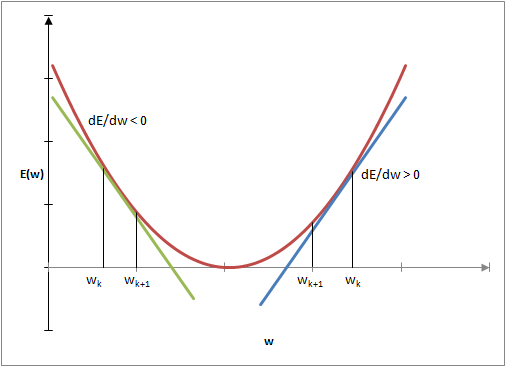
\includegraphics[width=0.8\textwidth]{images/gradient.png}
	\caption{Funkcja kosztu}
	\label{fig:gradient}
\end{figure}

\subsubsection*{Algorytm Levenberga-Marquardta}
Podczas gdy wcześniej nie została określona konkretna funkcji celu, tak w przypadku algorytmu Levenberga-Marquardta funkcją celu jest błąd średniokwadratowy (sum-of squares error, Mean Squared Error, MSE)\cite{Bishop}.
\begin{equation}
	\label{wzor:mse}
	E = \frac{1}{2} \sum_{n=1}^N(e_n)^2 = \frac{1}{2} \sum_{n=1}^N(y_n - \tilde{y_n})^2
\end{equation}
gdzie $e_n$ jest błędem n-tego wzorca, $y_n$ n-tym wzorcem, $\tilde{y_n}$ wyjściem sieci dla n-tego wzorca.

Zakładając, że aktualnie jesteśmy w punkcie $w_{i}$ i chcemy przemieścić się do punktu $w_{i+1}$, który jest niedaleko oddalony od $w_{i}$, w celu obliczenia nowej wartości błędu $e$ możemy skorzystać z rozwinięcia w szereg Taylora:
\begin{equation}
	\label{wzor:blad_lm}
	e(w_{i+1}) = e(w_{i}) + Z(w_{i+1} - w_{i})
\end{equation}
gdzie $Z \equiv \nabla e$. Po podstawieniu równania \ref{wzor:blad_lm} do równania \ref{wzor:mse} wzór na błąd średniokwadratowy może zostać zapisany jako:
\begin{equation}
	\label{wzor:mse2}
	E = \frac{1}{2}[e(w_{i}) + Z(w_{i+1} - w_{i})]^2
\end{equation}
Chcą zminimalizować równanie \ref{wzor:mse2} ze względu na zmienną $w_{i+1}$ otrzymujemy wzór:
\begin{equation}
	w_{i+1} = w_{i} - (Z^TZ)^{-1}Z^Te(w_{i})
\end{equation}
Jednak taki sposób obliczania $w_{i+1}$ może powodować, że krok $w_{i+1} - w_{i}$ będzie duży a wtedy liniowa aproksymacja szeregiem Taylora może stać się niedokładna. Z tego powodu algorytm Levenberga-Marquardta korzysta ze zmodyfikowanej funkcji celu w postaci:
\begin{equation}
	\label{wzor:mse_lm}
	E = \frac{1}{2}(e(w_{i}) + Z(w_{i+1} - w_{i}))^2 + \lambda (w_{i+1} - w_{i})^2
\end{equation}
Chcą zminimalizować równanie \ref{wzor:mse_lm} otrzymujemy ostatecznie równanie opisujące sposób obliczania wag w kolejnych iteracjach dla algorytmu Levenberga-Marquardta:
\begin{equation}
	w_{i+1} = w_{i} -(Z^TZ + \lambda I)^{-1}Z^Te(w_{i})
\end{equation}
gdzie $I$ jest macierzą jednostkową. Wartość $\lambda$ zmienia się w trakcie obliczania kolejnych wartości $w_{i+1}$. Jeśli błąd $E$ zmniejsza się wartość $\lambda$ jest zmniejszana o określony współczynnik. W przypadku wzrostu wartości błędu wartość $\lambda$ jest zwiększana o określony współczynnik oraz ponownie przyjmowana jest wartość $w_i$.



\newpage
\section{Selekcja funkcji bazowych oparta o metodę GOFR}
W przypadku sieci RBF problem może stanowić wybór odpowiednich funkcji bazowych oraz odpowiedniej ich ilości. Zbyt mała ilość funkcji nie pozwoli na wystarczające zminimalizowanie błędu sieci na zbiorze uczącym. Z kolei zbyt duża ilość funkcji może doprowadzić do problemu nadmiernego dopasowania a co za tym idzie sieć traci zdolność do generalizacji. Jedną z metod rozwiązania tego problemu jest zastosowanie metody GOFR opartej o metodę OLS (Orthogonal Least Square). 

\subsection{Selekcja oparta o ortogonalizację oraz metodę najmniejszych kwadratów}
Jedną z metod selekcji najbardziej znaczących funkcji bazowych jest metoda oparta o metodę najmniejszych kwadratów oraz ortogonalizację (OLS)\cite{Chen}. Metoda ta umożliwia określenie wkładu każdej funkcji bazowej i wybranie tych najbardziej istotnych. Mając dany wektor wag sieci $w = [w_0, w_1, \hdots, w_K]^T$ oraz wektor danych uczących $d = [d_1, d_2, \hdots, d_p]^T$ można zapisać macierz G w postaci:
\begin{equation}
G = \begin{bmatrix}
\phi_{11} & \phi_{21} & \hdots & \phi_{K1} \\
\phi_{12} & \phi_{22} & \hdots & \phi_{K2} \\
\hdots    & \hdots    & \hdots & \hdots    \\
\phi_{1p} & \phi_{2p} & \hdots & \phi_{Kp}
\end{bmatrix}
\end{equation}
gdzie $\phi_{ji}$ oznacza odpowiedź i-tej funkcji radialnej na j-ty wzorzec uczący. Oznaczając przez $g_i = [g_{i1}, g_{i2}, \hdots, g_{ip}]^T$ odpowiedź i-tej funkcji radialnej na wszystkie wzorce uczące można macierz G przedstawić w postaci:
\begin{equation}G = [g_1, g_2, \hdots, g_K] \end{equation}
Dla takich oznaczeń, dla sieci RBF można zapisać następujące równanie:
\begin{equation}
\label{wzor:ofr_rbf}
d = Gw + e\end
{equation}
gdzie $e$ jest błędem niedopasowania sieci. Ortogonalizacja macierzy G pozwala na określenie osobno wpływu każdej funkcji $g_i$ na wartość części pożądanej energii zdefiniowanej jako $(Gw)^2$ \cite{Osowski}. Dzięki temu możliwa jest selekcja najbardziej istotnych funkcji bazowych oraz znaczne ograniczenie ilości funkcji tworzących sieć. Sama ortogonalizacja może zostać dokonana różnymi metodami z czego często stosowaną jest metoda Grama-Schmidta, gdzie w procesie ortogonalizacji macierzy $G$ powstaje macierz ortogonalna $Q$ oraz macierz górnotrójkątna $A$.
\begin{equation}G = QA\end{equation}
\begin{equation}
A = \begin{bmatrix}
1      & a{12}  & a{13}  & \hdots & a_{1K} \\
0      & 1      & a{23}  & \hdots & a_{2K} \\
\hdots & \hdots & \hdots & \hdots & \hdots \\
0      & 0      & 0      & 0      & 1     
\end{bmatrix}
\end{equation}
Po procesie ortogonalizacji oraz wprowadzając nowe oznaczenie $b = Aw$ można zapisać nową postać równania \ref{wzor:ofr_rbf}:
\begin{equation}
	\label{wzor:ofr_rbf2}
	d = QAw + e = Qb + e
\end{equation}
Rozwiązując równanie \ref{wzor:ofr_rbf2} metodą najmniejszych kwadratów otrzymujemy:
\begin{equation}
	b = (QQ^T)^{-1}Q^Td
\end{equation}
Mając dane $b$ oraz $A$ jesteśmy wstanie określić wektor wag $w = A^{-1}b$.
Jak wspomniano wcześniej wartość pożądana energii jest określona jako $(Gw)^2$. Na tej podstawie można zdefiniować wzór określający udział danej funkcji w ogólnym bilansie energii jako:
\begin{equation}
	\epsilon_i = \frac{b_i^2q_i^Tq_i}{d^Td}
\end{equation}

Warunek stopu metody może zostać określony m. in. poprzez doprowadzenie do sytuacji gdzie wartość sumaryczna energii wnoszonej przez wszystkie funkcje będzie bliska jedności, czyli:
\begin{equation}
	1 - \sum_{i=1}^N \epsilon_i < \delta
\end{equation}
gdzie $\delta$ jest z góry ustaloną wielkością warunkując koniec algorytmu.

Jak wspomniano wcześniej ortogonalizacja może zostać wykonana różnymi metodami, jednak omówiona zostanie metoda ortogonalizacji Grama-Schmidta ze względu na jej popularność. Stosując algorytm ortogonalizacji Grama-Schmidta można dokonać rozkładu QR macierzy A, gdzie macierz Q jest macierzą ortogonalną zaś macierz R jest macierzą górnotrójkątną z jedynkami na diagonali. Algorytm takiego rozkładu można przedstawić w sposób następujący\cite{Bernardelli}:
\begin{equation}
	\begin{array}{l}
	q_1 = a_1 \\
	q_k = a_k - \sum_{j=1}^{k-1} r_{jk}q_j = a_k - \sum_{j=1}^{k-1} \frac{<a_k,q_j>}{<q_j,q_j>} q_j, \quad 2 \leq l  \leq n 
\end{array}
\end{equation}
$\frac{<a_k,q_j>}{<q_j,q_j>} q_j$ jest rzutowaniem ortogonalnym wektora $a_k$ na wektor $q_j$.

Graficzna reprezentacja procesu ortogonalizacji dla dwóch pierwszych kroków przedstawiona jest na rysunku \ref{fig:gram}. Mając wybrany wektor $u_1$ (literą $e$ oznaczono znormalizowany wektor $u$) należy dokonać projekcji (rzutu ortogonalnego) kolejnego wektora na przestrzeń rozpięta przez wszystkiego ortogonalne wektory (w tym przypadku tylko wektor $u_1$). Różnica wektora ortogonalizowanego oraz projekcji wektora ortogonalizowanego ($proj_{u_1}v_2$)na przestrzeń rozpiętą przez wektory ortogonalne pozwala uzyskać nam kolejny wektor ortogonalny ($u_2$).
\begin{figure}[ht!]
	\centering
	
	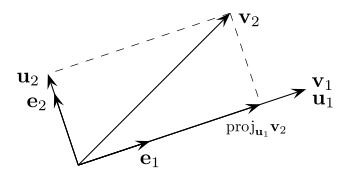
\includegraphics[scale=0.7]{images/GramSchmidt.png}
	\caption{Proces ortogonalizacji dla dwóch pierwszych kroków metody Grama-Schmidta \\
	\footnotesize {\textit{źródło:} http://commons.wikimedia.org/wiki/File:Gram\%E2\%80\%93Schmidt\_process.svg}}
	\label{fig:gram}	

\end{figure}

Funkcje wybiera się spośród wcześniej wygenerowanej biblioteki funkcji. Metoda ta zapewnia wybór najbardziej optymalnego zbioru funkcji z biblioteki. Jednak aby wybór ten był optymalny konieczne jest wygenerowanie odpowiedniej biblioteki, która może zawierać znaczną ilość funkcji bazowych przez co proces uczenia się sieci może stać się nieefektywny. Rozwiązaniem w tym przypadku jest zastosowanie metody GOFR

\subsection{Selekcja oparta o uogólnioną regresję postępującą z ortogonalizacją (GOFR)}
Metoda GOFR oparta jest na metodzie OLS\cite{Duboisa}. Modyfikację w stosunku do metody OLS stanowi optymalizacja dokonywana na etapie selekcji każdej funkcji bazowej. Optymalizacja ta polega na minimalizacji błędu sieci na zbiorze uczącym (np. zdefiniowanego jako MSE) poprzez odpowiedni dobór parametrów każdej wybranej funkcji. Optymalizacja taka może zostać przeprowadzona np. jedną z metod gradientowych.

Porównanie obu metod przedstawia schemat z rysunku \ref{ofr_and_gofr}. Linią przerywaną zaznaczony jest krok specyficzny dla metody GOFR. Optymalizacja pozwala na zmniejszenie ilości funkcji tworzących bibliotekę. Dzieje się tak dzięki temu, że po wyborze odpowiedniej funkcji algorytm zmodyfikuje parametry wybranej funkcji tak aby zminimalizować błąd. W przypadku algorytmu opartego o OLS parametry funkcji były stałe a ilość funkcji tworzących bibliotekę musiała być duża w celu zapewnienia odpowiednio wysokiego prawdopodobieństwa wyboru optymalnych funkcji bazowych.

\begin{figure}[ht!]
	\centering
	
	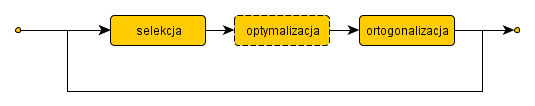
\includegraphics[scale=0.7]{images/ofr_and_gofr.png}
	\caption{Schemat algorytmu OFR oraz GOFR}
	\label{ofr_and_gofr}	

\end{figure}

\clearpage
\section{Identyfikacja systemu opisanego równaniem \mbox{Van der Pola}}

Równanie Van der Pola to równanie różniczkowe wyrażone wzorem:
\begin{equation}
	\label{wzor:van_der_pol}
	y''(t) - \mu(1 - y^2(t))y'(t) + y(t) = 0
\end{equation}

Równanie Van der Pola aktualnie jest często brane pod uwagę jako podstawowy model procesu oscylacji w fizyce, elektronice, biologii, neurologii, socjologii i ekonomii\cite{Tsatsos}.

Identyfikację systemu opisanego równaniem \ref{wzor:van_der_pol} (dla $\mu = 1$) oparto o sieć RBF i metodę GOFR selekcji funkcji bazowych. Strukturę zaproponowanej sieci przedstawia rysunek~\ref{fig:rbf}.
\begin{figure}[ht!]
	\centering
	
	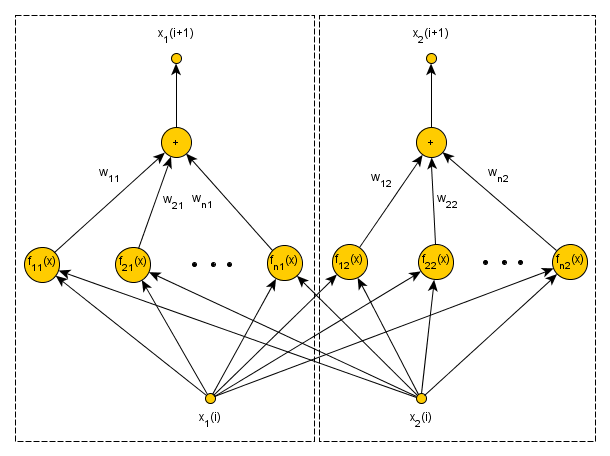
\includegraphics[width = \textwidth]{images/rbf.png}
	\caption{Schemat zaprojektowanej sieci RBF}
	\label{fig:rbf}	

\end{figure}
Wejście sieci stanowią $x_1 = y(t)$ oraz $x_2 = y'(t)$, czyli aktualny stan obiektu. Wyjściem sieci jest stan obiektu w kolejnym kroku. Jak można zauważyć sieć została podzielona na dwie do pewnego stopnia niezależne części - każde z wejść posiada oddzielny zestaw funkcji RBF. W związku z tym każda z części sieci była uczona oddzielnie (dla tych samych danych uczących). 

Zbiór danych uczących sieć neuronową wygenerowano rozwiązując równanie metodą Runge-Kutty IV rzędu dla warunków początkowych [$y(0)=0,y'(0)=2$], kroku metody $h=0.1$, w~przedziale $t \in [0,40]$. Równanie różniczkowe \ref{wzor:van_der_pol} drugiego rzędu zapisano w postaci układu dwóch równań różniczkowych pierwszego rzędu:
\begin{equation}
	\begin{array}{l}
    y'(t)  = y_1 \\
    y_1'(t) = (1-y_1^2)y-y_1
    \end{array}
\end{equation}

Powstała w wyniku rozwiązania równania Van der Pola trajektoria, wykres funkcji $y(t)$ oraz jej pierwszej pochodnej $y'(t)$ przedstawione są odpowiednio na rysunkach \ref{img:traj}, \ref{img:func} oraz \ref{img:first_deriv}. Dane powstałe w wyniku rozwiązania równania zostały użyte jako zbiór danych uczących.

\begin{figure}[ht!]
	\centering

	\subfloat[Trajektoria]
	{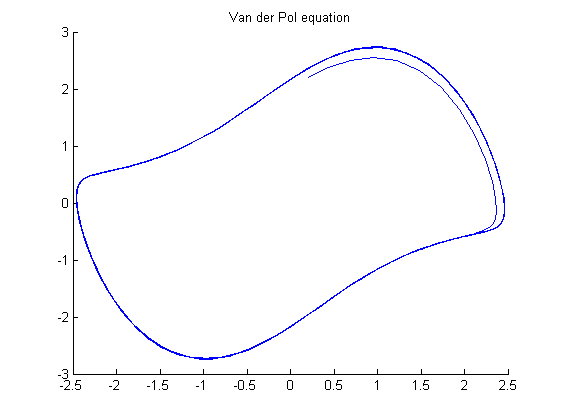
\includegraphics[width=0.5\textwidth]
	{images/trajectory.png}
	\label{img:traj}}
	\subfloat[Wykres funkcji $y(t)$]
	{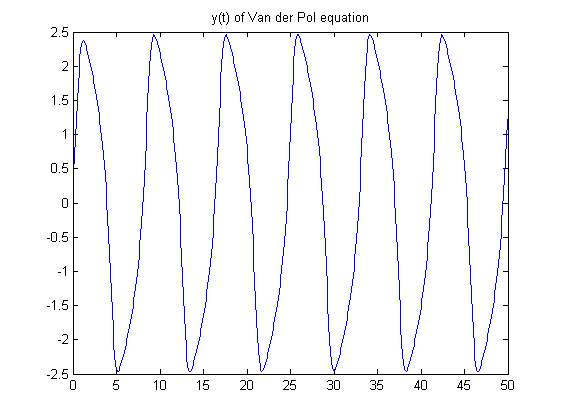
\includegraphics[width=0.5\textwidth]
	{images/signal.png}
	\label{img:func}}
	
	\subfloat[Wykres pierwszej pochodnej $y'(t)$]
	{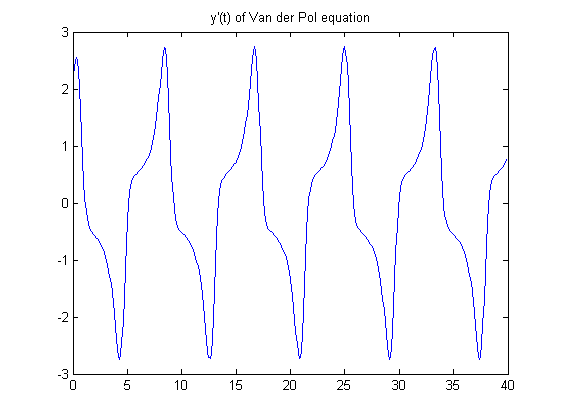
\includegraphics[width=0.45\textwidth]
	{images/first_deriv.png}
	\label{img:first_deriv}}
	
	\caption{Wykresy powstałe w wyniku rozwiązania równania różniczkowego Van der Pola dla warunków początkowych [$y(0)=0,y'(0)=2$]}
\end{figure}

Kolejnym etapem było stworzenie odpowiedniej biblioteki funkcji RBF. W tym celu najpierw wygenerowano bibliotekę 115 funkcji RBF postaci:
\begin{equation}
	\label{wzor:rbf_2d}
	f(x_1(t),x_2(t),c_1,c_2,\sigma) = e^{-\frac{(x_1(t)-c_1)^2 + (x_2(t)-c_2)^2}{2 \sigma^2}}\
\end{equation} gdzie: \\
$x_1(t) = y(t)$ \\
$x_2(t) = y'(t)$ \\

Generowanie biblioteki odbywało się poprzez wybór równomiernie rozłożonych w przestrzeni dwuwymiarowej $D = [min(x_1),max(x_1)] \times [min(x_2),max(x_2)]$ centrów. Dla każdego kolejnego poziomu generowania biblioteki funkcji, nowe centra $c_1$ oraz $c_2$ były wybierane poprzez dwukrotnie zagęszczenie punktów w każdej z osi oraz zmniejszanie szerokości funkcji gaussa $\sigma$ o połowę. Centra dla tak wygenerowanych funkcji przedstawia rysunek \ref{img:rbf_centers}. Ilość poziomów ograniczono do trzech generując w ten sposób 115 funkcji RBF.

\begin{figure}[ht!]
	\centering	
	
	\subfloat
	{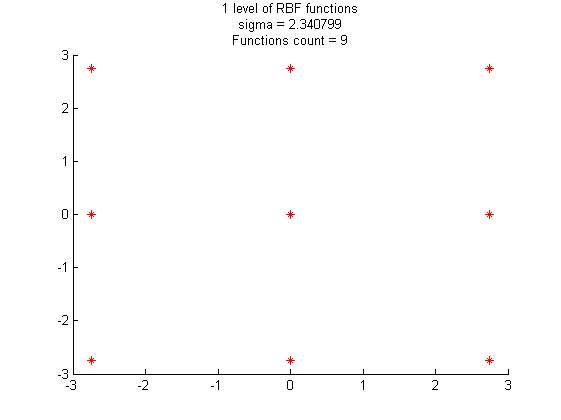
\includegraphics[width=0.33\textwidth]
	{images/centers1.png}}
	\subfloat
	{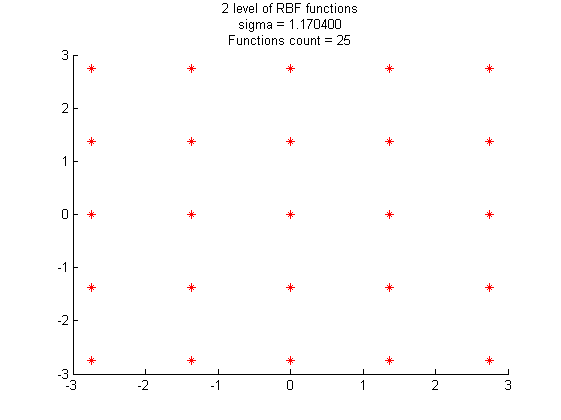
\includegraphics[width=0.33\textwidth]
	{images/centers2.png}}
	\subfloat
	{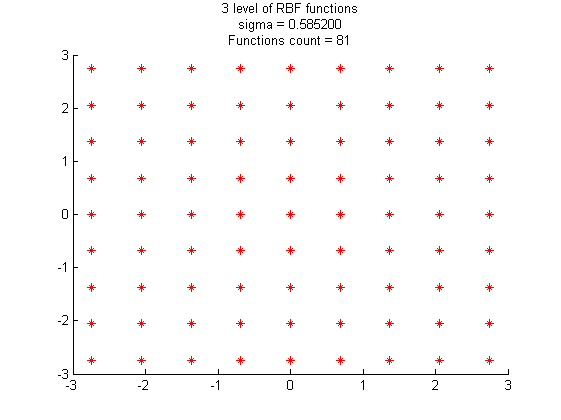
\includegraphics[width=0.33\textwidth]
	{images/centers3.png}}

	\caption{Centra wygenerowanych funkcji RBF}
	\label{img:rbf_centers}
\end{figure}

Następnie dokonano selekcji najbardziej istotnych funkcji z biblioteki wykorzystując metodę GOFR. Po selekcji każdej z funkcji dokonywana jest optymalizacja wybranej funkcji metodą Levenberga-Marquardta. Sieć neuronowa o funkcjach bazowych zdefiniowanych wzorem \ref{wzor:rbf_2d} realizuje funkcję:
\begin{equation}
	\tilde{y} = \sum_{i=1}^N w_i f_i(x_1,x_2,c_1,c_2,\sigma_i)
\end{equation}
Optymalizowano następujące parametry sieci RBF: $c_1$, $c_2$, $\sigma$ oraz $w$. W celu skorzystania z~metody Leveberga-Marquardta konieczne jest określenie gradientu funkcji błędu $e = y - \tilde{y}$ oraz jej pochodnych cząstkowych. Funkcja błędu $e$ jest wyrażona wzorem:
\begin{equation}
	e = y - \tilde{y} = y - w f(x_1,x_2,c_1,c_2,\sigma) = y - w e^{-\frac{(x_1-c_1)^2 + (x_2-c_2)^2}{2 \sigma^2}} 
\end{equation}
Gradient $e$ wynosi zatem:
\begin{equation}
\begin{bmatrix}
	\frac{\partial e}{\partial w} \\
	\frac{\partial e}{\partial \sigma} \\
	\frac{\partial e}{\partial c_1} \\
	\frac{\partial e}{\partial c_2}
\end{bmatrix} = 
\begin{bmatrix}
	f(\cdot) \\
	w f(\cdot) \frac{(x_1 - c_1)^2 + (x_2 - c_2)^2}{\sigma^3}\\
	w f(\cdot) \frac{(x_1 - c_1)}{\sigma^2}\\
	w f(\cdot) \frac{(x_2 - c_2)}{\sigma^2}	
\end{bmatrix}
\end{equation}

W przypadku zwiększania się błędu na zbiorze uczącym parametr $\lambda$ ze wzoru \ref{wzor:mse_lm} był zwiększany 10-krotnie, w przypadku zmniejszania się błędu parametr $\lambda$ był zmniejszany 10-krotnie. Warunek stopu został ustalony tak aby błąd średniokwadratowy dla każdego z wyjść sieci był mniejszy od 1e-6. 






\clearpage
\section{Wyniki identyfikacji obiektu opisanego równaniem Van der Pola}

Osiągnięcie błędu średniokwadratowego poniżej 1e-6 udało się osiągnąć dla 24 funkcji bazowych dla $y(t)$ (błąd równy = 6.8925e-7) oraz 25 funkcji bazowych dla $y'(t)$ (błąd równy = 7.2683e-7). Na rysunkach \ref{fig:signal_approx_a}, \ref{fig:signal_approx_b} oraz rysunkach \ref{fig:deriv_approx_a}, \ref{fig:deriv_approx_b} zostały przedstawione odpowiednio: aproksymacja funkcji $y(t)$ oraz aproksymacja pierwszej pochodnej $y'(t)$ równania Van der Pola  dla pierwszych sześciu iteracji. Jak można zauważyć kształt funkcji $y(t)$ oraz pochodnej $y'(t)$ jest dokładnie odwzorowany już po selekcji kilku pierwszych funkcji. Dzieje się tak ze względu na to, że algorytm selekcji funkcji bazowych GOFR wybiera funkcje wnoszące największy wkład energii w kolejnych iteracjach. Kolejne wybierane funkcje mają coraz mniejsze znaczenie w odwzorowywaniu obiektu opisanego równaniem Van der Pola.

\begin{figure}[ht!]
	\centering

	\subfloat
	{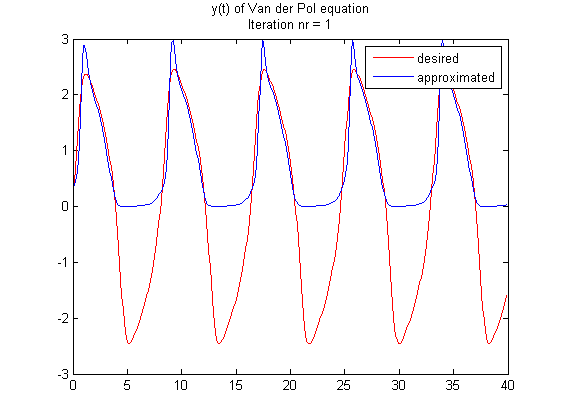
\includegraphics[width=0.5\textwidth]
	{images/signal_iter1.png}}
	\subfloat
	{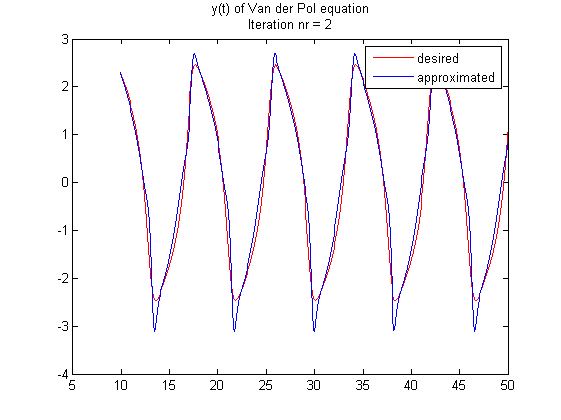
\includegraphics[width=0.5\textwidth]
	{images/signal_iter2.png}}
	
	\subfloat
	{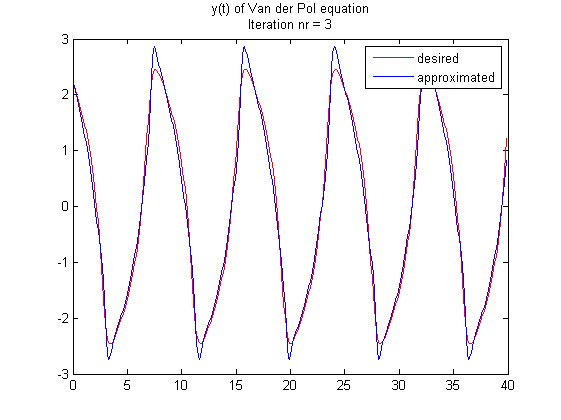
\includegraphics[width=0.5\textwidth]
	{images/signal_iter3.png}}
	\subfloat
	{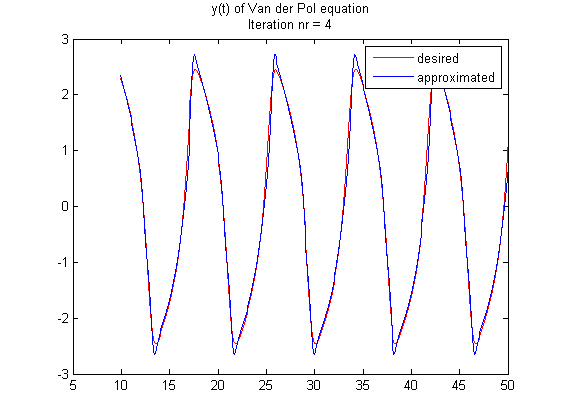
\includegraphics[width=0.5\textwidth]
	{images/signal_iter4.png}}

	\caption{Aproksymacja funkcji y(t) po selekcji funkcji numer 1-4}		
	\label{fig:signal_approx_a}		
\end{figure}

\begin{figure}[ht!]
	\centering

	\subfloat
	{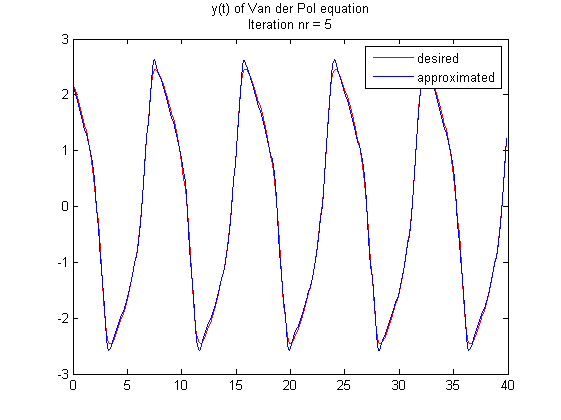
\includegraphics[width=0.5\textwidth]
	{images/signal_iter5.png}}
	\subfloat
	{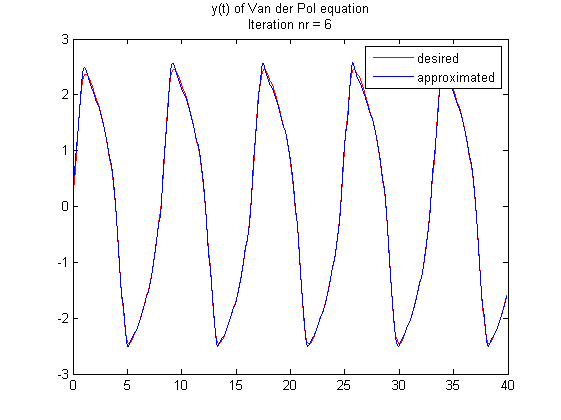
\includegraphics[width=0.5\textwidth]
	{images/signal_iter6.png}}	

	\caption{Aproksymacja funkcji y(t) po selekcji funkcji numer 5-6}		
	\label{fig:signal_approx_b}		
\end{figure}

\begin{figure}[ht!]
	\centering
	
	\subfloat
	{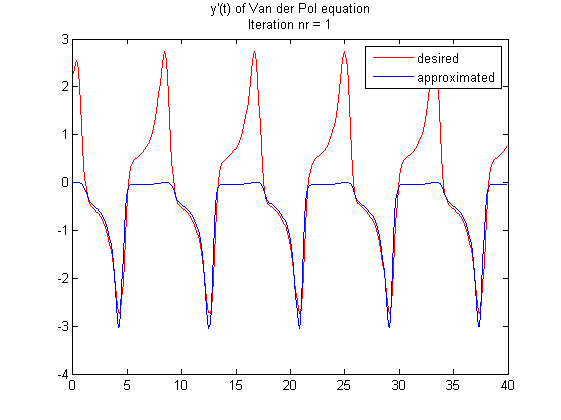
\includegraphics[width=0.5\textwidth]
	{images/deriv_iter1.png}}
	\subfloat
	{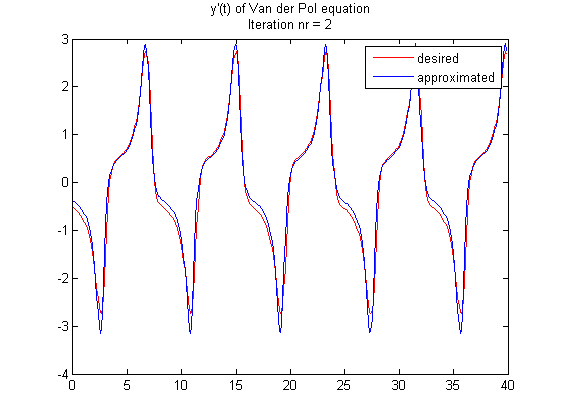
\includegraphics[width=0.5\textwidth]
	{images/deriv_iter2.png}}
	
	\subfloat
	{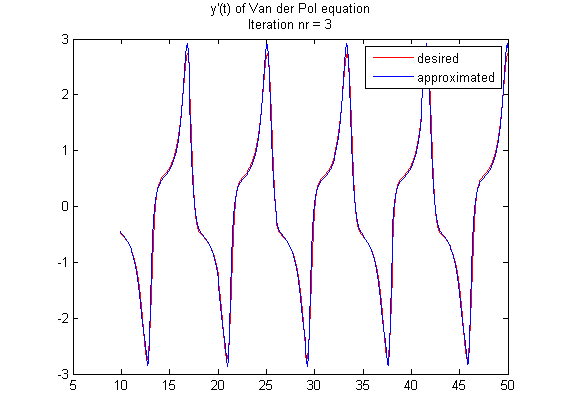
\includegraphics[width=0.5\textwidth]
	{images/deriv_iter3.png}}
	\subfloat
	{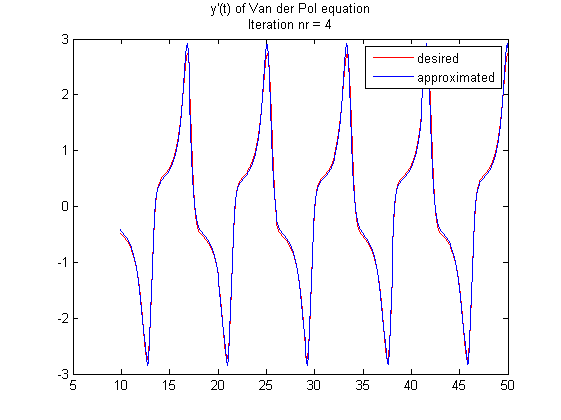
\includegraphics[width=0.5\textwidth]
	{images/deriv_iter4.png}}

	\caption{Aproksymacja funkcji y'(t)  po selekcji funkcji numer 1-4}		
	\label{fig:deriv_approx_a}
\end{figure}

\begin{figure}[ht!]
	\centering
	
	\subfloat
	{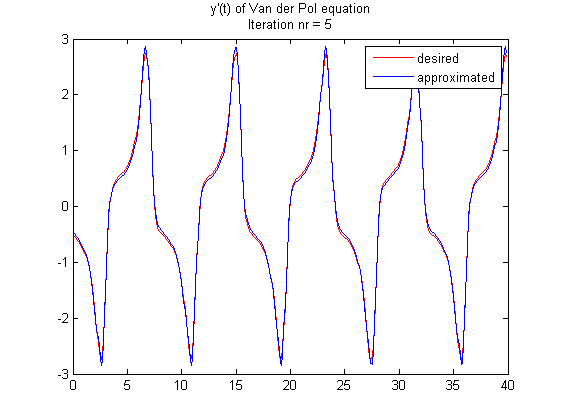
\includegraphics[width=0.5\textwidth]
	{images/deriv_iter5.png}}
	\subfloat
	{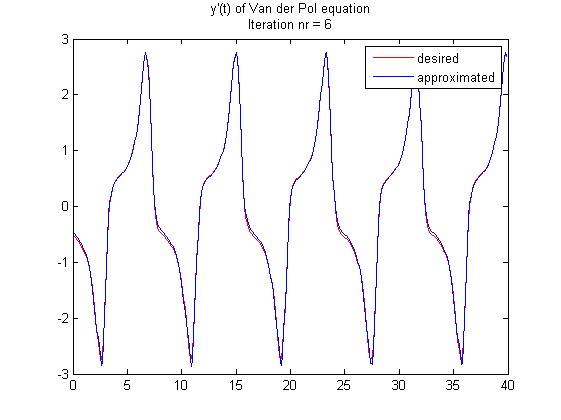
\includegraphics[width=0.5\textwidth]
	{images/deriv_iter6.png}}	
	
	\caption{Aproksymacja funkcji y'(t) po selekcji funkcji numer 5-6}		
	\label{fig:deriv_approx_b}
\end{figure}

Rysunek \ref{img:approximated} przedstawia aproksymację równania Van der Pola przez wytrenowaną sieć.

\begin{figure}[ht!]
	\centering

	\subfloat
	{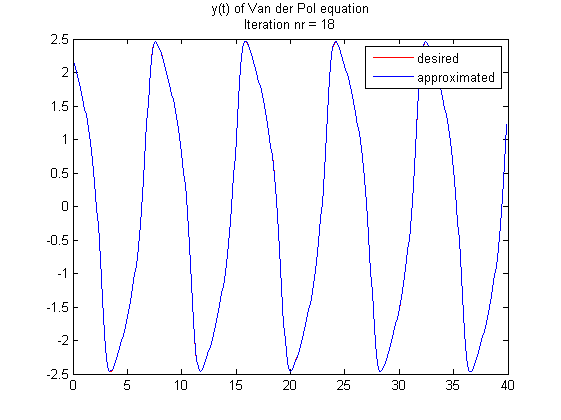
\includegraphics[width=0.5\textwidth]
	{images/signal_approx.png}}
	\subfloat
	{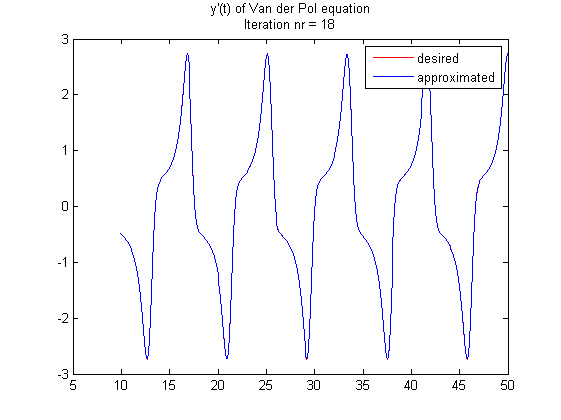
\includegraphics[width=0.5\textwidth]
	{images/deriv_approx.png}}	
	
	\subfloat
	{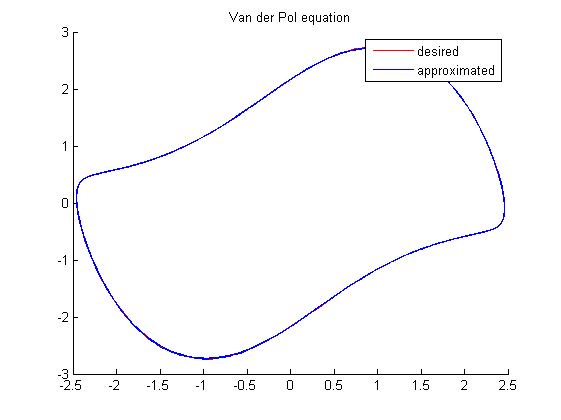
\includegraphics[width=0.5\textwidth]
	{images/trajectory_approx.png}}

	\caption{Sygnał zadany oraz aproksymowany przez wytrenowaną sieć RBF $t \in [0,40]$}
	\label{img:approximated}
\end{figure}


W tabeli \ref{tab:rbf_tabela_x1} zostały zebrane dane na temat wybranych funkcji RBF oraz błąd średniokwadratowy aproksymacji funkcji $y(t)$ równania Van der Pola po selekcji kolejnych funkcji RBF.
\begin{table}[ht!]
\centering

\begin{tabular}{ | c| c| c| c| c| c| c| }
\hline
number & indeks RBF & centrum 1 & centrum 2 & szerokość $\sigma$ & energia      & błąd MSE \\ \hline    
	
 1 &  32  &  2.9948  &  0.7222  &  1.5295  &  4.7410e-1 & 1.5872e+0 \\
 2 &   2  & -5.8209  & -1.0474  &  2.6805  &  4.9905e-1 & 8.1038e-2 \\
 3 &   8  &  7.0671  &  1.4665  &  3.8568  &  1.5418e-2 & 3.4504e-2 \\
 4 &  52  & -2.2270  &  3.0342  &  0.7155  &  5.3306e-3 & 1.8416e-2 \\
 5 &  15  & -1.0761  & -3.1178  &  1.0496  &  4.5295e-3 & 4.7450e-3 \\
 6 &  60  & -1.3884  &  2.1498  &  0.5889  &  7.8749e-4 & 2.3682e-3 \\
 7 & 103  &  2.0854  &  0.7488  &  0.6221  &  4.1060e-4 & 1.1290e-3 \\
 8 &  47  & -1.9902  & -0.6401  &  0.5865  &  1.0880e-4 & 8.0058e-4 \\
 9 & 106  &  1.9631  &  3.4429  &  0.4688  &  1.1553e-4 & 4.5188e-4 \\
10 &  20  &  0.6923  & -3.9854  &  1.3350  &  4.7597e-5 & 3.0823e-4 \\
11 &  68  & -0.4170  &  1.0838  &  0.6116  &  3.8596e-5 & 1.9174e-4 \\
12 & 109  &  2.7940  & -1.5663  &  0.5293  &  1.5792e-5 & 1.4408e-4 \\
13 &  62  & -0.7083  & -2.5993  &  0.5065  &  8.2334e-6 & 1.1923e-4 \\
14 &  79  &  0.5131  &  2.2032  &  0.2673  &  1.8315e-5 & 6.3952e-5 \\
15 &   5  & -0.0016  &  0.0540  &  2.3580  &  4.6821e-6 & 4.9821e-5 \\
16 &   4  &  0.0067  & -2.7505  &  2.3463  &  5.5652e-6 & 3.3024e-5 \\
17 &  92  &  1.4041  & -0.7927  &  0.5950  &  4.2814e-6 & 2.0102e-5 \\
18 &   6  & -0.0072  &  2.7806  &  2.3611  &  1.4043e-6 & 1.5864e-5 \\
19 &  14  & -2.7163  &  2.7149  &  1.1521  &  1.0246e-6 & 1.2771e-5 \\
20 & 102  &  1.9456  &  0.0229  &  0.5151  &  2.3885e-6 & 5.5625e-6 \\
21 &  94  &  1.3554  &  0.6871  &  0.5818  &  4.3525e-7 & 4.2489e-6 \\
22 & 115  &  2.9594  &  2.8968  &  0.5772  &  5.1100e-7 & 2.7066e-6 \\
23 &  28  &  1.3478  &  1.3509  &  1.1561  &  4.2283e-7 & 1.4304e-6 \\
24 &  35  & -2.7401  & -2.7393  &  0.5862  &  2.4558e-7 & 6.8925e-7 \\
    \hline
\end{tabular}

\caption{Wybrane funkcje RBF dla y(t)}
\label{tab:rbf_tabela_x1}
\end{table}

W tabeli \ref{tab:rbf_tabela_x2} zostały zebrane dane na temat wybranych funkcji RBF oraz błąd średniokwadratowy aproksymacji pochodnej $y'(t)$ równania Van der Pola po selekcji kolejnych funkcji RBF.

\begin{table}[ht!]
\centering

\begin{tabular}{ |c| c| c| c| c| c| c| }
\hline
numer & indeks RBF & centrum 1 & centrum 2 & szerokość $\sigma$ & energia      & błąd MSE    \\ \hline    
    1 &  20 &   1.1446 &  -5.7343  &  2.0595 &   4.9501e-1 & 9.4653e-1 \\
    2 &  24 &  -0.5846 &   5.1218  &  2.1860 &   4.8488e-1 & 3.7690e-2 \\
    3 &  71 &   0.3756 &  -3.5358  &  0.8221 &   1.1585e-2 & 1.5975e-2 \\
    4 &  55 &  -1.3838 &  -1.3455  &  0.5934 &   4.5029e-3 & 7.5351e-3 \\
    5 & 105 &   2.6435 &   2.2556  &  0.6908 &   1.9649e-3 & 3.8522e-3 \\
    6 &  18 &  -1.7286 &   1.9662  &  0.9173 &   9.8872e-4 & 1.9989e-3 \\
    7 &  31 &   2.7142 &  -1.5228  &  1.1111 &   4.3126e-4 & 1.1906e-3 \\
    8 &  35 &  -2.4433 &  -2.8083  &  0.4078 &   1.8653e-4 & 8.4097e-4 \\
    9 &  34 &   2.4846 &   2.5536  &  1.0744 &   1.3652e-4 & 5.8508e-4 \\
   10 &   4 &  -0.0373 &  -2.1985  &  2.0320 &   8.6977e-5 & 4.2205e-4 \\
   11 &  51 &  -2.0368 &   2.1029  &  0.5648 &   1.0665e-4 & 2.2215e-4 \\
   12 &  44 &  -2.3244 &  -3.0361  &  0.5831 &   4.1302e-5 & 1.4473e-4 \\
   13 &  87 &   0.6683 &   2.1058  &  0.5772 &   2.7287e-5 & 9.3585e-5 \\
   14 & 108 &   2.5990 &  -1.9039  &  0.5283 &   1.8039e-5 & 5.9773e-5 \\
   15 &   5 &  -0.0008 &   0.0006  &  2.3321 &   1.0989e-5 & 3.9175e-5 \\
   16 &  66 &  -0.8763 &   0.2859  &  0.5596 &   4.5942e-6 & 3.0564e-5 \\
   17 &  56 &  -1.2921 &  -0.5707  &  0.4300 &   4.8491e-6 & 2.1475e-5 \\
   18 & 112 &   2.9438 &   0.5975  &  0.4572 &   3.6241e-6 & 1.4682e-5 \\
   19 &  54 &  -1.3559 &  -2.0394  &  0.5777 &   2.9742e-6 & 9.1075e-6 \\
   20 &  97 &   1.6974 &   3.4300  &  0.7467 &   1.8032e-6 & 5.7277e-6 \\
   21 &  86 &   0.7040 &   1.3515  &  0.5634 &   8.1315e-7 & 4.2035e-6 \\
   22 &  63 &  -0.6910 &  -2.0473  &  0.5768 &   6.0731e-7 & 3.0652e-6 \\
   23 &  39 &  -3.3163 &   0.0390  &  0.6737 &   3.4036e-7 & 2.4273e-6 \\
   24 & 111 &   2.3400 &   0.0310  &  0.4559 &   7.2918e-7 & 1.0605e-6 \\
   25 &  53 &  -1.3701 &  -2.7398  &  0.5851 &   1.7802e-7 & 7.2683e-7 \\
    \hline
\end{tabular}

\caption{Wybrane funkcje RBF dla y'(t)}
\label{tab:rbf_tabela_x2}
\end{table}

\clearpage

Błąd średniokwadratowy w funkcji wybranych funkcji RBF przedstawia rysunek \ref{img:prediction_error} natomiast rysunek \ref{img:energy} przedstawia energię jaką wnosi każda kolejna wybrana funkcja. Jak można zauważyć główny wpływ na wartość błędu oraz energii mają dwie pierwsze wybrane funkcje. Wraz z wyborem kolejnych funkcji błąd oraz energia wnoszona przez wybraną funkcję spadają w przybliżeniu logarytmicznie. Zieloną linią na wykresie \ref{img:prediction_error} została oznaczona wartość MSE, która jest warunkiem stopu uczenia sieci.

\begin{figure}[ht!]
	\centering

	{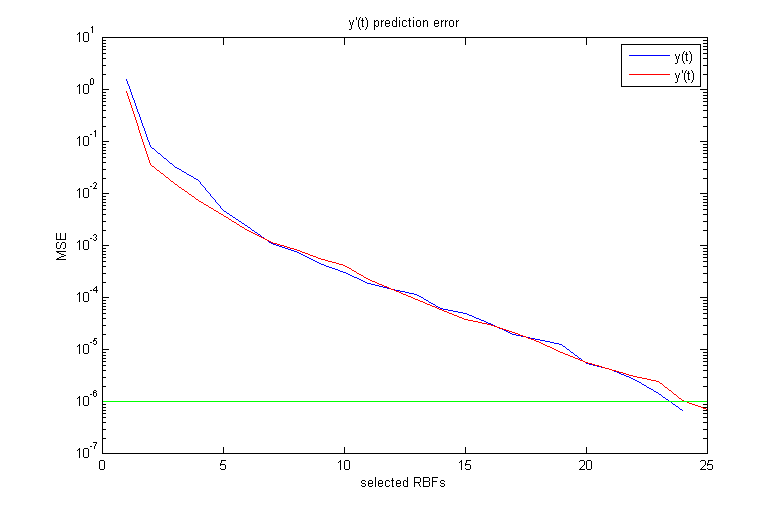
\includegraphics[width=\textwidth]
	{images/prediction_error.png}}

	\caption{Błąd MSE w funkcji wybranych funkcji RBF}
	\label{img:prediction_error}
\end{figure}


\begin{figure}[ht!]
	\centering

	{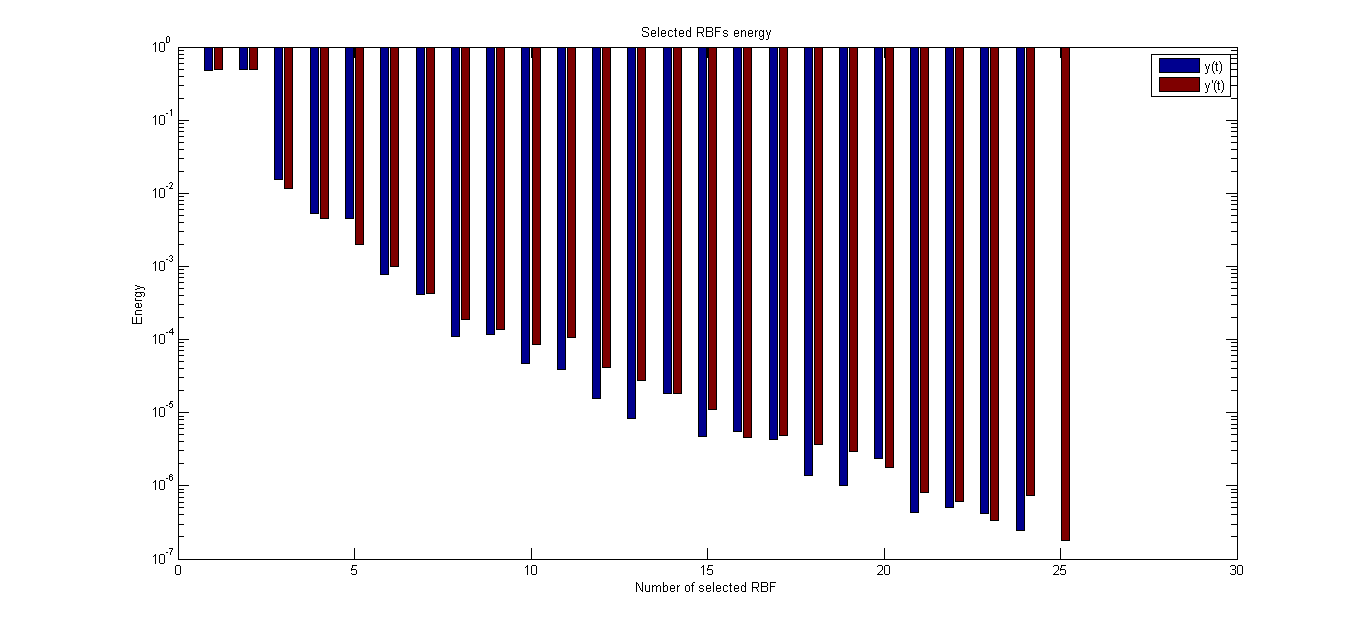
\includegraphics[width=0.8\textwidth]
	{images/rbfs_energy.png}}

	\caption{Energia wnoszona przez kolejne wybrane funkcji RBF}
	\label{img:energy}
\end{figure}

Po etapie trenowania sieci RBF sprawdzono zdolność tej sieci do predykcji. Predykcja na 100 kroków do przodu została przedstawiona na rysunku~\ref{img:predicted}. Jak można zauważyć sieć dobrze modeluje obiekt opisany równaniem Van der Pola. Błąd średniokwadratowy dla wyznaczania $y(t)$ wyniósł  5.6108e-5, natomiast błąd predykcji wyznaczania $y'(t)$ wyniósł 9.4761e-5.

\begin{figure}[ht!]
	\centering

	\subfloat
	{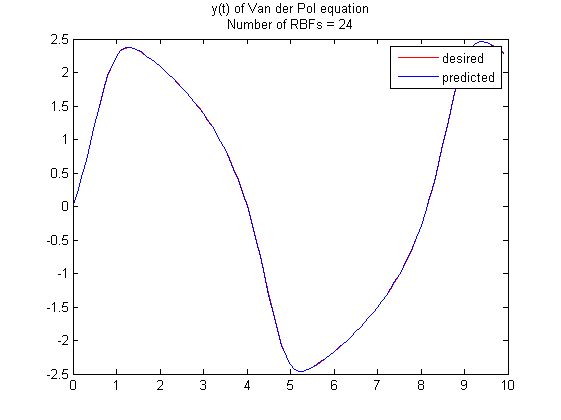
\includegraphics[width=0.45\textwidth]
	{images/signal_pred100.png}}
	\subfloat
	{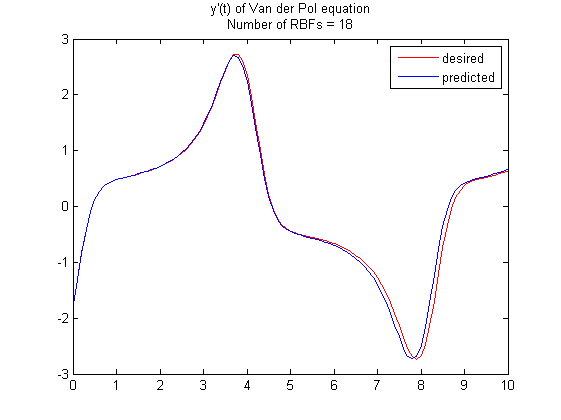
\includegraphics[width=0.45\textwidth]
	{images/deriv_pred100.png}}	
	
	\subfloat
	{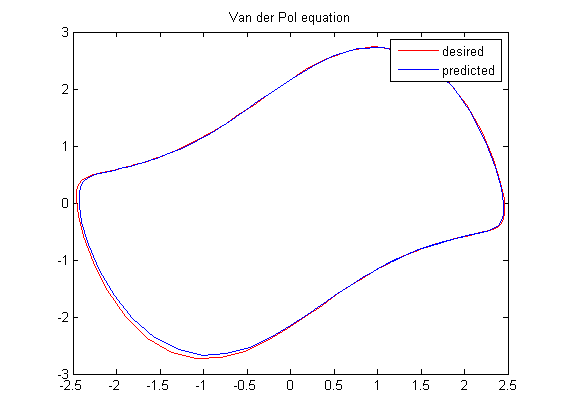
\includegraphics[width=0.45\textwidth]
	{images/trajectory_pred100.png}}

	\caption{Sygnał zadany oraz przewidywany przez wytrenowaną sieć RBF $t \in [0,10]$}
	\label{img:predicted}
\end{figure}

Trudno jest jednak dokładniej określić jakość predykcji na podstawie rysunku \ref{img:predicted} ze względu na nieznaczne różnice w wartości zadanej oraz wartości przewidywanej przez sieć w wyniku czego sygnał zadany oraz przewidywany pokrywają się. Aby można było dokładnie określić odstępstwo wartość przewidywanej od wartości rzeczywistej na rysunku \ref{img:err100_x} został przedstawiony błąd predykcji w funkcji w kolejnych krokach. Wartość bezwzględna błędu wyznaczenia $y(t)$ nie przekracza wartości 0.02. Maksymalny błąd wyznaczenia $y'(t)$ jest nieznacznie większy i nie przekracza wartości 0.03. Na tej podstawie można stwierdzić, że dla 100 kroków w przód sieć spełnia swoje zadanie. 

\begin{figure}[ht!]
	\centering

	\subfloat
	{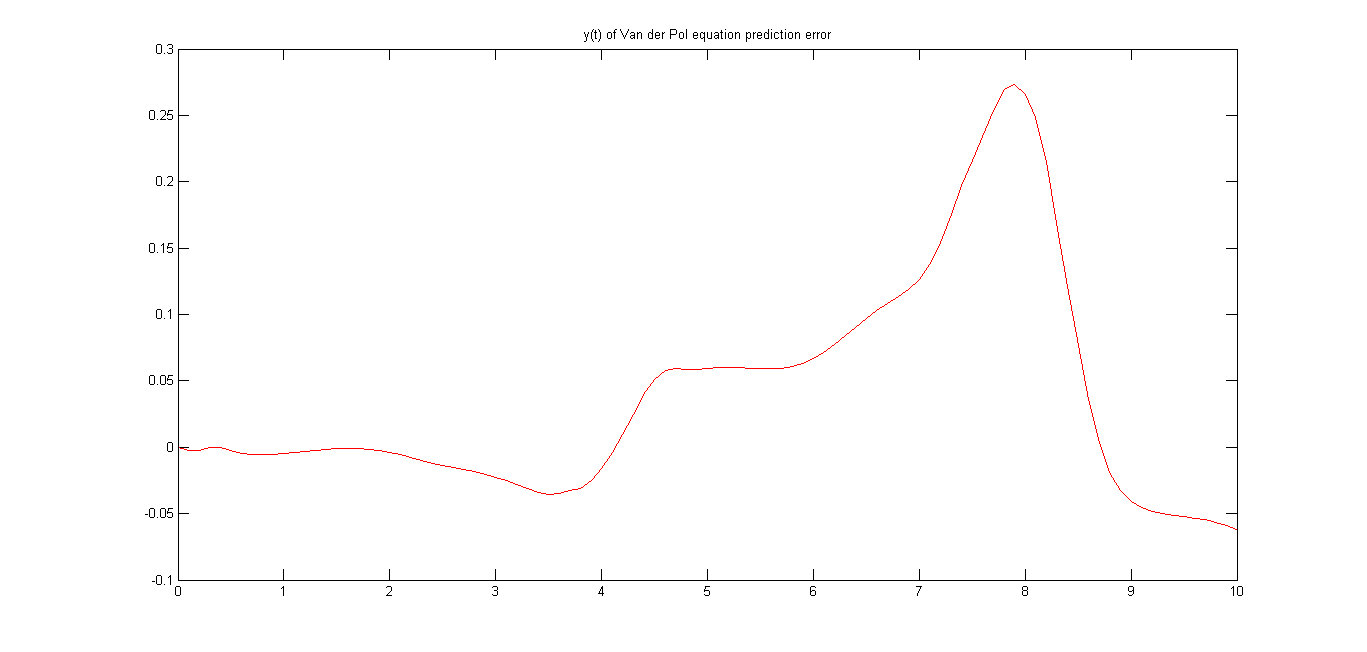
\includegraphics[width=0.5\textwidth]
	{images/err100_x1.png}}
	\subfloat
	{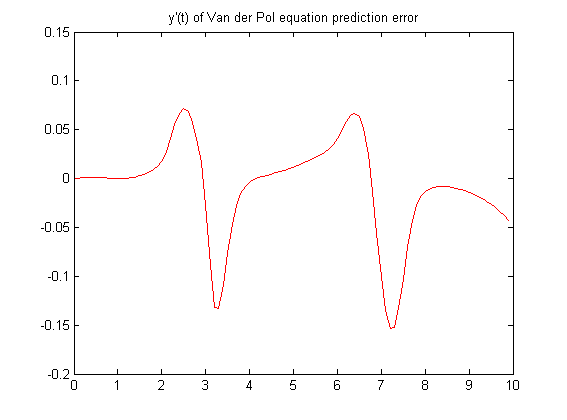
\includegraphics[width=0.5\textwidth]
	{images/err100_x2.png}}	
	

	\caption{Błąd predykcji w funkcji czasu $t \in [0,10]$}
	\label{img:err100_x}
\end{figure}


Następnie zdecydowana się na sprawdzenie jakości predykcji w 5-krotnie dłuższym przedziale czasu $t \in [0, 50]$. Na rysunku \ref{img:predicted2} został przedstawiany sygnał rzeczywisty oraz przewidywany. Jak można zauważyć jakość predykcji jest nadal dobra ale podobnie jak wcześniej trudno jest określić dokładnie błąd między wartością przewidywaną a rzeczywistą. Nieznaczną rozbieżność można zauważyć na wykresie trajektorii. Błąd średniokwadratowy dla wyznaczania $y(t)$ wyniósł  1.9873e-4, natomiast błąd wyznaczania $y'(t)$ wyniósł 3.0130e-4, czyli kilkukrotnie wzrósł w stosunku do błędu dla 5-kronie krótszego okresu predykcji.

\begin{figure}[ht!]
	\centering

	\subfloat
	{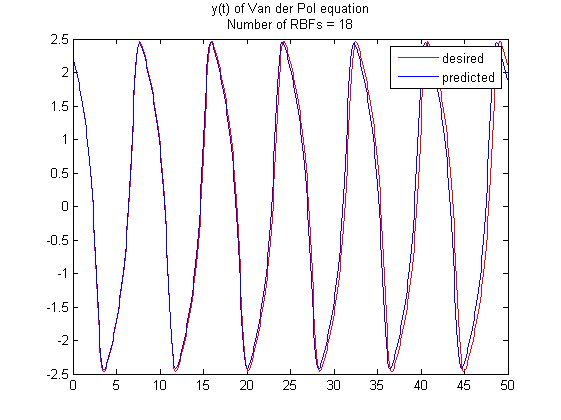
\includegraphics[width=0.5\textwidth]
	{images/signal_pred400.png}}
	\subfloat
	{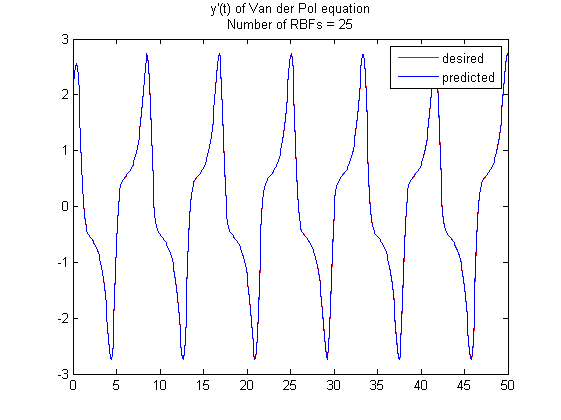
\includegraphics[width=0.5\textwidth]
	{images/deriv_pred400.png}}	
	
	\subfloat
	{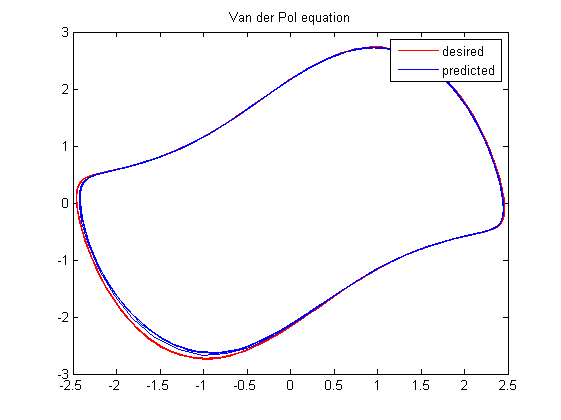
\includegraphics[width=0.5\textwidth]
	{images/trajectory_pred400.png}}

	\caption{Sygnał zadany oraz przewidywany przez wytrenowaną sieć RBF $t \in [0,50]$}
	\label{img:predicted2}
\end{figure}

Aby dokładniej określić jakość predykcji w przedziale czasu $t \in [0, 50]$ ponownie skorzystano z wykresu błędu predykcji dla kolejnych kroków. Jak można zauważyć wraz z oddalaniem się od punktu początkowego błąd predykcji rośnie. Dzieje się tak ze względu na akumulację błędu. Należy zaznaczyć jednak, że odchylenie od wartości zadanej dla 500 kroków dla $y(t)$ nie przekracza wartości 0.04 natomiast dla $y'(t)$ nie przekracza wartości 0.07 co pozwala stwierdzić, że nawet dla tak długiego okresu czasu sieć spełnia swoje zadanie.

\begin{figure}[ht!]
	\centering

	\subfloat
	{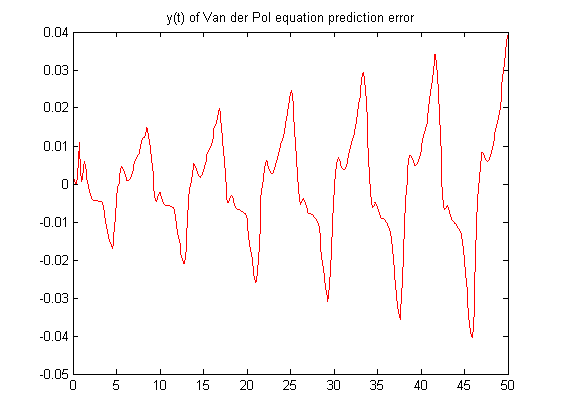
\includegraphics[width=0.5\textwidth]
	{images/err1000_x1.png}}
	\subfloat
	{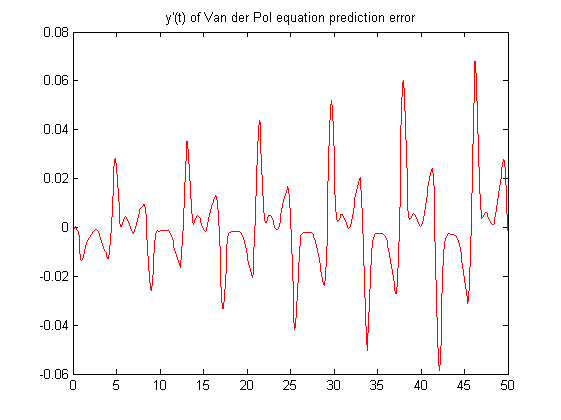
\includegraphics[width=0.5\textwidth]
	{images/err1000_x2.png}}	
	

	\caption{Błąd predykcji w funkcji czasu $t \in [0,50]$}
	\label{img:err}
\end{figure}

Do tej pory badana była jedynie predykcja dla tych samych warunków początkowych dla jakich sieć została wytrenowana. Jednak aby model był dobrze odwzorowany należałoby sprawdzić czy sieć jest zdolna do predykcji dla szerszego zakresu warunków początkowych. W tym celu została przeprowadzona predykcja dla 440 różnych wartości początkowych równomiernie rozłożonych w przestrzeni $[-2,2] \times [-2,2]$ dla 100 kroków w przód. Jakość predykcji została oceniona na podstawie błędu średniokwadratowego. Wykres obrazujący jakość predykcji w zależności od warunków początkowych przedstawia rysunek \ref{img:err_initial}.

\begin{figure}[ht!]
	\centering

	\subfloat
	{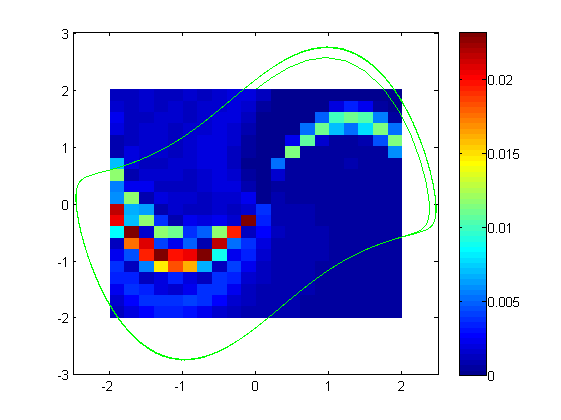
\includegraphics[width=0.5\textwidth]
	{images/figure_signal.png}}
	\subfloat
	{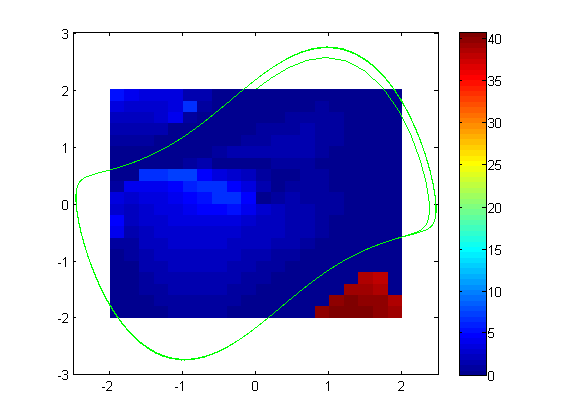
\includegraphics[width=0.5\textwidth]
	{images/figure_deriv.png}}	
	

	\caption{Błąd predykcji w zależności od warunków początkowych $t \in [0,50]$}
	\label{img:err_initial}
\end{figure}

Jak można zauważyć sieć dobrze modeluje obiekt nie tylko dla wcześniej wybranego warunku początkowego ale również dla warunków początkowych położonych w pobliżu trajektorii powstałej w wyniku rozwiązania równania Van der Pola z warunkiem początkowym jaki został wybrany w celu stworzenia zbioru uczącego. Rysunek \ref{img:err_initial} może być mylący ze względu na skalę barw jaka została użyta dla określenia błędu pochodnej - zakres błędu dla różnych warunków początkowych jest zdecydowanie większy dla $y'(t)$ niż dla $y(t)$ (maksymalny błąd MSE dla $y(t)$ wynosi 13.6417 natomiast dla $y'(t)$ wynosi 40.6341). Po analizie okazało się, że istnieje 16 (na 440) warunków początkowych dla których błąd średniokwadratowy jest większy od 10 . Z tego względu dla lepszego zobrazowania rozkładu błędu zastąpiono wszystkie 16 wartości błędu większe od 10 błędem = 10 i ponownie wykreślono rozkład błędu MSE $y'(t)$ w zależności od warunków początkowych. Przedstawiony jest on na rysunku \ref{img:err_initial_new}.

\begin{figure}[ht!]
	\centering

	\subfloat
	{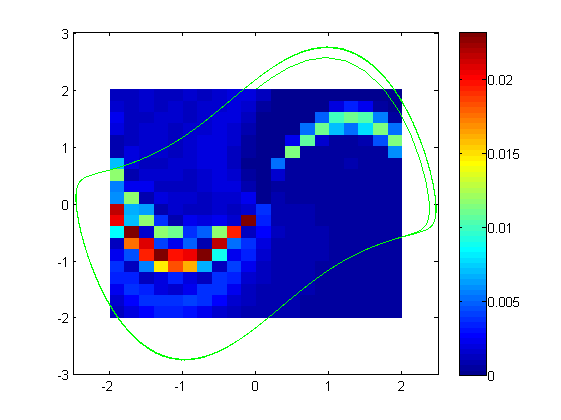
\includegraphics[width=0.5\textwidth]
	{images/figure_signal.png}}
	\subfloat
	{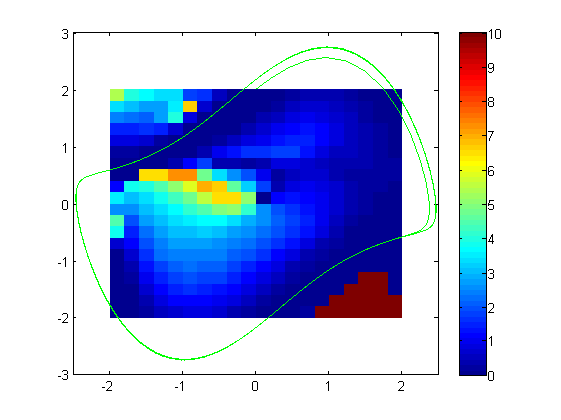
\includegraphics[width=0.5\textwidth]
	{images/figure_deriv_new.png}}	
	

	\caption{Błąd predykcji w zależności od warunków początkowych $t \in [0,50]$ po odrzuceniu wartości skrajnych błedu mse $y'(t)$}
	\label{img:err_initial_new}
\end{figure}

Po odrzuceniu skrajnych wartości wykres rozkładu błędu $y'(t)$ znacznie bardziej przypomina wykres rozkładu błędu $y(t)$. Dla większości warunków początkowych sieć jednak nie jest wstanie dobrze modelować obiektu. Ustalając akceptowalność predykcji, dla której błąd MSE był mniejszy niż 0.01, sieć była wstanie poprawnie modelować obiekt dla 51 z 440 warunków początkowych. Stworzony model zatem jest odpowiedni jedynie dla określonego zbioru warunków początkowych co może być akceptowalne jeśli jesteśmy w stanie założyć, że modelowany obiekt będzie działał jedynie dla takich warunków początkowych. Aby sieć neuronowa była wstanie modelować równanie w szerszym zakresie warunków początkowym potrzebne są kolejne dane. W tym celu wygenerowano 80 trajektorii powstałych w wyniku rozwiązania równania Van der Pola dla warunków początkowych równomiernie rozłożonych w przestrzeni $[-2,2] \times [-2,2]$ w przedziale czasu $t \in [0, 40]$ z krokiem $h=0.1$. Zdecydowano się na zmodyfikowanie warunku stopu do postaci $mse < 1e-5$ ze względu na znaczne zwiększenie się zbioru uczącego a co za tym idzie znacznie wydłużenie uczenia się sieci.
Osiągnięcie błędu średniokwadratowego poniżej 1e-5 udało się osiągnąć dla 25 funkcji bazowych dla funkcji $y(t)$ (błąd równy = 9.5037e-6) oraz 26 funkcji bazowych dla pochodnej $y'(t)$ (błąd równy = 7.9001e-6), czyli wykorzystując jedynie jedną funkcję bazową więcej dla każdej z części sieci. Należy jednak w tym miejscu przypomnieć, że warunkiem stopu było uzyskanie błędu średniokwadratowego 10-krotnie większego niż miało to miejsce w przypadku wcześniejszym. 

W tabeli \ref{tab:rbf_tabela2_x1} zostały zebrane dane na temat wybranych funkcji RBF oraz błąd średniokwadratowy aproksymacji $y(t)$ po selekcji kolejnych funkcji RBF.

\begin{table}[ht!]
\centering

\begin{tabular}{ |c| c| c| c| c| c| c| }
\hline
numer & indeks RBF & centrum 1 & centrum 2 & szerokość $\sigma$ & energia      & błąd MSE    \\ \hline    
    1 &  12 &  -4.8953 &  -0.9105 &   2.0586  &  4.7050e-1 & 1.5515e+0 \\
    2 &   8 &   5.4193 &   0.9971 &   2.5798  &  5.0360e-1 & 7.5903e-2 \\
    3 &   2 &  -4.6034 &  -0.8540 &   3.0277  &  1.4313e-2 & 3.3965e-2 \\
    4 &   5 &   0.0222 &  -0.2106 &   3.2317  &  9.8758e-3 & 5.0279e-3 \\
    5 &  97 &   2.0527 &   3.4549 &   0.7361  &  1.0031e-3 & 2.0888e-3 \\
    6 &  77 &   0.1850 &   1.2900 &   0.6728  &  3.6159e-4 & 1.0293e-3 \\
    7 &  84 &   0.8268 &  -0.0171 &   0.6789  &  9.3702e-5 & 7.5471e-4 \\
    8 & 103 &   2.0429 &   0.6027 &   0.5178  &  8.7412e-5 & 4.9858e-4 \\
    9 &  53 &  -1.4953 &  -3.9012 &   0.6884  &  5.9932e-5 & 3.2298e-4 \\
   10 &  56 &  -1.5088 &  -0.7513 &   0.6456  &  4.0396e-5 & 2.0461e-4 \\
   11 &  60 &  -1.6142 &   2.5627 &   0.6911  &  2.5830e-5 & 1.2893e-4 \\
   12 & 108 &   3.2889 &  -1.8451 &   0.4369  &  8.0323e-6 & 1.0539e-4 \\
   13 &  57 &  -1.7669 &   0.1593 &   0.3909  &  6.2747e-6 & 8.7008e-5 \\
   14 &  69 &  -0.7720 &   2.5602 &   0.7003  &  4.4067e-6 & 7.4096e-5 \\
   15 &  11 &  -2.7698 &  -1.4594 &   1.1633  &  3.9520e-6 & 6.2516e-5 \\
   16 &  27 &   1.5564 &   0.1463 &   1.2159  &  3.2820e-6 & 5.2899e-5 \\
   17 &  30 &   3.2537 &  -3.1569 &   1.1834  &  3.6829e-6 & 4.2108e-5 \\
   18 &  88 &   0.7869 &   3.5360 &   0.4310  &  4.5237e-6 & 2.8853e-5 \\
   19 & 105 &   2.6917 &   2.6612 &   0.5780  &  1.8611e-6 & 2.3400e-5 \\
   20 &  40 &  -3.9490 &   1.0595 &   0.7024  &  1.0632e-6 & 2.0285e-5 \\
   21 & 109 &   3.3322 &  -1.6728 &   0.6157  &  6.1811e-7 & 1.8474e-5 \\
   22 &  38 &  -4.0090 &  -0.9720 &   0.7012  &  7.5296e-7 & 1.6267e-5 \\
   23 &  36 &  -3.8224 &  -2.8683 &   0.7438  &  1.0858e-6 & 1.3086e-5 \\
   24 &  65 &  -0.8844 &  -0.9351 &   0.6755  &  6.7549e-7 & 1.1107e-5 \\
   25 &  58 &  -1.5267 &   0.4323 &   0.5790  &  5.4706e-7 & 9.5037e-6 \\    \hline
\end{tabular}

\caption{Wybrane funkcje RBF dla y(t)}
\label{tab:rbf_tabela2_x1}
\end{table}


W tabeli \ref{tab:rbf_tabela2_x2} zostały zebrane dane na temat wybranych funkcji RBF oraz błąd średniokwadratowy aproksymacji $y'(t)$ po selekcji kolejnych funkcji RBF.

\begin{table}[ht!]
\centering

\begin{tabular}{ |c| c| c| c| c| c| c| }
\hline
numer & indeks RBF & centrum 1 & centrum 2 & szerokość $\sigma$ & energia      & błąd MSE    \\ \hline    
    1 &  24 &  -1.1250  &  5.6516  &  2.0361  &  4.7516e-1 & 9.8511e-1   \\
    2 &  20 &   0.5488  & -4.9698  &  2.1518  &  5.0392e-1 & 3.9276e-2   \\
    3 &  78 &  -0.3925  &  3.5349  &  0.8580  &  1.2219e-2 & 1.6341e-2   \\
    4 & 104 &   1.8566  &  1.5269  &  0.6389  &  4.4165e-3 & 8.0511e-3   \\
    5 &  55 &  -2.6142  & -2.2752  &  0.7069  &  1.9361e-3 & 4.4172e-3   \\
    6 &  26 &   1.6316  & -1.7819  &  0.9866  &  1.0335e-3 & 2.4773e-3   \\
    7 &  13 &  -2.6461  &  0.9889  &  1.0006  &  3.2912e-4 & 1.8596e-3   \\
    8 &  71 &   0.4828  & -3.7540  &  0.7487  &  2.0188e-4 & 1.4807e-3   \\
    9 &  86 &   0.7849  &  1.5639  &  0.7424  &  1.9636e-4 & 1.1121e-3   \\
   10 & 115 &   2.9828  &  3.1229  &  0.5308  &  8.5215e-5 & 9.5215e-4   \\
   11 &  67 &  -0.6655  &  0.4598  &  0.6018  &  1.2760e-4 & 7.1264e-4   \\
   12 & 112 &   2.5479  &  0.7001  &  0.3633  &  7.6301e-5 & 5.6943e-4   \\
   13 & 105 &   2.8729  &  2.8243  &  0.7434  &  7.0644e-5 & 4.3683e-4   \\
   14 &  16 &  -1.4468  & -1.5020  &  1.1100  &  3.6943e-5 & 3.6749e-4   \\
   15 &  51 &  -2.5600  &  2.5033  &  0.6451  &  3.9223e-5 & 2.9387e-4   \\
   16 &  95 &   1.7201  &  1.7280  &  0.6390  &  2.2062e-5 & 2.5246e-4   \\
   17 & 109 &   2.9319  & -1.0482  &  0.4542  &  1.8539e-5 & 2.1767e-4   \\
   18 &  44 &  -2.0737  & -2.9877  &  0.4729  &  1.4993e-5 & 1.8953e-4   \\
   19 &   6 &  -0.0106  &  3.5027  &  2.6365  &  1.3682e-5 & 1.6385e-4   \\
   20 &   5 &   0.0097  &  0.0031  &  2.6574  &  2.0389e-5 & 1.2558e-4   \\
   21 &  32 &   3.3282  & -0.0031  &  1.2907  &  2.1197e-5 & 8.5791e-5   \\
   22 &  25 &   2.0450  & -3.8439  &  1.3209  &  1.6687e-5 & 5.4470e-5   \\
   23 &  50 &  -2.7665  &  1.9171  &  0.7318  &  1.5010e-5 & 2.6296e-5   \\
   24 &  97 &   2.0519  &  4.1067  &  0.7983  &  4.8446e-6 & 1.7203e-5   \\
   25 &  63 &  -0.8497  & -2.6336  &  0.6773  &  3.5100e-6 & 1.0615e-5   \\
   26 &  83 &   0.7341  & -0.7148  &  0.6868  &  1.4466e-6 & 7.9001e-6   \\
   \hline
\end{tabular}

\caption{Wybrane funkcje RBF dla y'(t)}
\label{tab:rbf_tabela2_x2}
\end{table}

\clearpage
 Następnie dokonano sprawdzenia czy sieć po zwiększeniu zbioru uczącego jest wstanie dobrze modelować układ dla różnych warunków początkowych. Wykres obrazujący jakość predykcji w zależności od warunków początkowych przedstawia rysunek \ref{img:err_initial2}.


\begin{figure}[ht!]
	\centering

	\subfloat
	{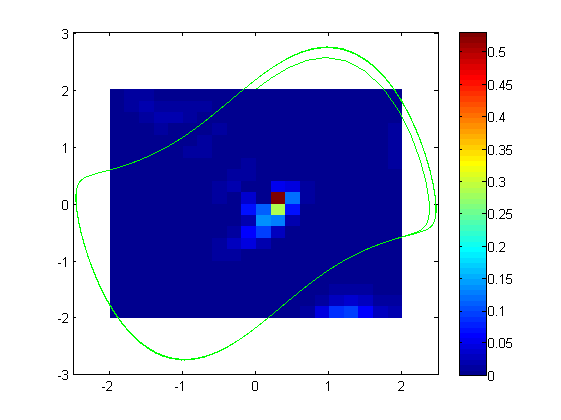
\includegraphics[width=0.5\textwidth]
	{images/figure_signal2.png}}
	\subfloat
	{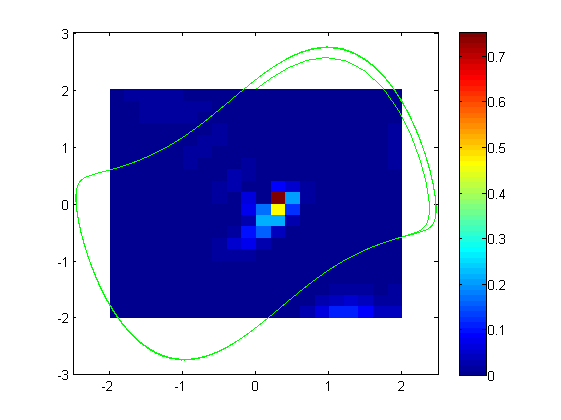
\includegraphics[width=0.5\textwidth]
	{images/figure_deriv2.png}}	
	

	\caption{Błąd predykcji w zależności od warunków początkowych $t \in [0,10]$}
	\label{img:err_initial2}
\end{figure}

Jak można zauważyć dla większości warunków początkowych sieć dobrze modeluje układ. Największa wartość błędu wynosiła odpowiednio 0.5292 dla $y(t)$ oraz 0.7508 dla $y'(t)$. W porównaniu do wartości maksymalnej wartości błędu dla sieci uczonej na podstawie danych z jednej trajektorii (maksymalny błąd mse dla $y(t)$ wynosił 13.6417 natomiast dla $y'(t)$ wynosił 40.6341) błąd średniokwadratowy zmalał kilkadziesiąt razy. Znacznie wzrosła też ilość warunków początkowych, dla których błąd MSE predykcji był mniejszy niż 0.01. Wartość ta wzrosła z 51 do 348 warunków początkowych.

\clearpage
\section{Podsumowanie oraz wnioski}

Celem pracy była próba identyfikacji nieliniowych obiektów dynamicznych z wykorzystaniem metody GOFR. Cel udało się zrealizować identyfikując obiekt dynamiczny opisany równaniem Van der Pola. Posiadając dane tylko z jednej trajektorii sieć była wstanie dobrze modelować obiekt dla różnych warunków początkowych. Predykcja na 500 kroków w przód skutkowała błędem średniokwadratowym w wyznaczeniu $y(t)$ równym 1.9873e-4, oraz błędem wyznaczania $y'(t)$ równym 3.0130e-4. Następnie aby zwiększyć jakość odwzorowania modelu obiektu dla szerszego zakresu punktów początkowych zwiększono zbiór danych uczących do 80 trajektorii. Po ponowny wytrenowaniu sieci okazało się, że jakość odwzorowania modelu dla szerokiego zakresu warunków początkowych uległa znacznemu polepszeniu.
Określając jako akceptowalną predykcje taką, dla której błąd mse < 0.01 dla $y(t)$ oraz $y'(t)$ jednocześnie, udało się uzyskać poprawną predykcję dla 348 na 440 warunków początkowych.

Czas uczenia sieci uległ jednak znacznemu wydłużeniu a ilość funkcji bazowych uległa zwiększeniu pomimo ustalania jako warunku stopu uzyskania błędu mse dziesięciokrotnie mniejszego. Pomimo zwiększenia zbioru uczącego dla części warunków początkowych sieć nadal nie najlepiej odwzorowywała obiekt dynamiczny.  Wartości początkowe dla których błąd był większy od gwarantującego poprawną predykcję były zgrupowane. Dalszą poprawę wyników mogłoby przynieść zwiększenie zbioru uczącego bądź zmniejszenie wartości mse jako warunku stopu. Jednym z ograniczeń takiej identyfikacji jest modelowanie obiektu dla z góry określonego kroku (dla identyfikowanego obiektu h = 0.1). Rozwiązanie takiego problemu zostało jednak zaproponowane w pracy Yi-Jen Wanga i Chin-Teng Lina\cite{Wang}. Wykorzystane w tym celu zostało połączenie metody Runge-Kutty oraz radialnej sieci neuronowej. Sieć przedstawioną w pracy można wykorzystać w tej metodzie tak aby umożliwić swobodny dobór kroku metody.

W pracy ''Structure-unknown non-linear dynamic systems: identification through neural networks''\cite{Masri} została podjęta próba identyfikacji dynamiki obiektu opisanego równaniem Van der Pola. Zastosowano tam sieć jednokierunkową, trzywarstową oraz algorytm propagacji wstecznej błędu. Nie zostały tam zamieszczone konkretne dane liczbowe ale oceniając identyfikację obiektu na podstawie zamieszczonych tam wykresów można ocenić jakościowo, że zaproponowany w pracy dyplomowej sposób identyfikacji oparty o sieć neuronową i metodę GOFR zdecydowanie lepiej spełnił swoje zadanie. 

Przedstawiona w pracy metoda sprawdziła się w identyfikacji dynamiki obiektu nieliniowego opisanego równaniem Van der Pola. W dalszych pracach można wykorzystać metodę GOFR do identyfikacji innych nieliniowych obiektów dynamicznych oraz zastosować ją w połączeniu z metodą Runge-Kutty.

% -------------------------- bibliografia ----------------------------
\clearpage

\addcontentsline{toc}{section}{Literatura}
\begin{thebibliography}{widest-label}

\bibitem{AK_RBG2002}Kharab A., Ronald B. Guenther, An introduction to numerical methods : a MATLAB approach, 2002, Chapman \& Hall/CRC

\bibitem{BCh_2001}Bogdan Choczewski (red.), Równania różniczkowe zwyczajne i cząstkowe. Zadania z matematyki, Kraków 2001, Wydawnictwa AGH

\bibitem{Osowski}Osowski S., Sieci neuronowe do przetwarzania informacji, Warszawa 2006, Oficyna Wydawnicza Politechniki Warszawskiej

\bibitem{Bishop}Bishop C. M., Neural Networks for Pattern Recognition, Oxford University Press, 1995 Oxford

\bibitem{Bartkowiak} Bartkowiak A., (Notatki do wykładu Sieci Neuronowe), Sieci RBF - o radialnych funkcjach bazowych, https://www.ii.uni.wroc.pl/~aba/teach/NN/w9rbf.pdf

\bibitem{Chen} Chen S., Cowan C. F. N., Grant P. M., Orthogonal Least Squares Learning Algorithm for Radial Basis Function Networks, IEEE, 1991

\bibitem{Duboisa} R. Duboisa, B. Queneta, Y. Faisandierb, G. Dreyfusa, Building meaningful representations for nonlinear modeling of 1d- and 2d-signals: applications to biomedical signals

\bibitem{Gutenbaum} J. Gutenbaum, Modelowanie systemów,

\bibitem{Kosinski} R. A. Kosiński, Sztuczne sieci neuronowe, Warszawa 2007, WNT

\bibitem{Bors} Bors Adrian G., Introduction of the Radial Basis Function (RBF) Networks, http://www-users.cs.york.ac.uk/adrian/Papers/Others/OSEE01.pdf

\bibitem{Bernardelli} http://akson.sgh.waw.pl/~mbernard/Dydaktyka/Rok\_2010\_11/WprowadzenieD oMetodNumerycznychLic\_1011\_let/Zajecia06.pdf

\bibitem{Palczewski} Palczewski A., Równania różniczkowe zwyczajne
Teoria i metody numeryczne z wykorzystaniem komputerowego systemu obliczeń symbolicznych, WNT 2004 Warszawa wyd. 2

\bibitem{Czemplik} Czemplik. A, Modele dynamiki układów fizycznych dla inżynierów
Zasady i przykłady konstrukcji modeli dynamicznych obiektów automatyki, 2008 WNT, Warszawa

\bibitem{Isermann} Rolf Isermann, Marco Münchhof, Identification of Dynamic Systems: An Introduction with Applications, Springer 2010

\bibitem{Wang} Wang, Runge–Kutta Neural Network for Identification
of Dynamical Systems in High Accuracy

\bibitem{Masri} Masri, Structure-unknown non-linear dynamic
systems: identification through neural
networks

\bibitem{Tsatsos} Marios Tsatsos, Dissertation: Theoretical and Numerical Study of
the Van der Pol equation, Thessaloniki, July 2006, Aristotle University of Thessaloniki
School of Sciences

\bibitem{Jankowski} Jankowski
\end{thebibliography}

\clearpage
\addcontentsline{toc}{section}{Dodatek A: Kod źródłowy programu}
\section*{Dodatek A: Kod źródłowy programu}

\textit{van\_der\_pol.m}

\begin{lstlisting}
% Function solving Van der Pol equations usign 4-th order Runge-Kutta method
%
% t_end - end of time period for solution (time starts from 0)
% h     - time step
% y0    - init values

function [t,y] = rk_van_der_pol(t_end, h, y0)

    % Runge-Kutta general formula
    % y_{i+1} = y_i + 1/6*(k_1 + 2k_2 + 2k_3 + k_4), i = 0,1,2,...
    % k_1 = hf(x_i,y_1)
    % k_2 = hf(x_i + 1/2h, y_1 + 1/2k_1)
    % k_3 = hf(x_i + 1/2h, y_1 + 1/2k_2)    
    % k_4 = hf(x_i + h, y_1 + k_3)
    
    t = 0:h:t_end;
    n = length(t);
    h = 0.1;

    y = zeros(n, 2);
    y(1, 1) = y0(1);
    y(1, 2) = y0(2);
    
    % Van der Pol equation 
    % y''(t) - (1 - y^2(t)) * y'(t) + y(t) = 0;
    % y'(t)  = y(2)
    % y''(t) = (1-y(1)^2)*y(2)-y(1)

    for i = 1:n-1
        k1 = h*(y(i,2));
        k2 = h*(y(i,2)+0.5*k1);
        k3 = h*(y(i,2)+0.5*k2);
        k4 = h*(y(i,2)+k3);
        y(i+1,1) = y(i,1)+(k1+2*k2+2*k3+k4)/6;
        
        y1 = y(i,1);
        y2 = y(i,2);
        k1 = h*((1-y1^2)*y2-y1);
        y1 = y(i,1)+0.5*k1;
        y2 = y(i,2)+0.5*k1;
        k2 = h*((1-y1^2)*y2-y1);
        y1 = y(i,1)+0.5*k2;
        y2 = y(i,2)+0.5*k2;
        k3 = h*((1-y1^2)*y2-y1);
        y1 = y(i,1)+k3;
        y2 = y(i,2)+k3;
        k4 = h*((1-y1^2)*y2-y1);
        y(i+1,2) = y(i,2)+(k1+2*k2+2*k3+k4)/6;

    end
    
end

\end{lstlisting}

\textit{gofr.m}

\begin{lstlisting}
function [selected_rbfs, W, E_k, A_k, Q_k, B_k, centers, sigmas, G] =  gofr(X, y, G, centers, sigmas, K)

    rbf_number = length(centers);

    D = y;
    Q = zeros(size(G));
    Q_k = zeros(size(G));
    B = zeros(1,rbf_number);
    B_k = zeros(1,rbf_number);
    E = zeros(1,rbf_number);
    E_k = zeros(1,K);
    selected_rbfs = zeros(1,rbf_number);      % indexes of selected rbfs order by decreasing energy 

    A = cell(1,rbf_number);
    A_k = eye(rbf_number);
    for i = 1:rbf_number
        A{i} = eye(rbf_number);
    end

    % ----- selection of the most significant functions -----
    for k = 1:K
        % Gram-Schmidt orthogonalization
        for i = 1:rbf_number
           Q(:,i) = G(:,i);

           % if rbf is already selected function omit it 
           if ismember(i, selected_rbfs) == 1
               continue;
           end

           for j=1:k-1
                A{i}(j,k) = Q_k(:,j)'*G(:,i) / (Q_k(:,j)'*Q_k(:,j));
                Q(:,i) = Q(:,i) - A{i}(j,k)*Q_k(:,j);
           end

           B(i) = Q(:,i)'*D / (Q(:,i)'*Q(:,i));
           E(i) = B(i)^2*Q(:,i)'*Q(:,i) / (D'*D);   
        end

        % find RBF with maximum energy (save index and copy to Q_k matrix)
        [E_k(k) selected_rbfs(k)] = max(E);
        B_k(k) = B(selected_rbfs(k));
        A_k(:,k) = A{selected_rbfs(k)}(:,k);
        W = A_k\B_k';

        % ------ Levenberg-Marquardt -----
        Theta = [W(k); sigmas(selected_rbfs(k)); centers(1, selected_rbfs(k)); centers(2, selected_rbfs(k))];

        y_rbf = 0;
        for j = 1:k
            y_rbf = y_rbf + W(j) * gaussian_2D(X, sigmas(selected_rbfs(j)), centers(:,selected_rbfs(j))');
        end
        

        lambda = 0.1;
        Theta_old = Theta;
        N = 100;   % maximum iterations of gradient method
        err = zeros(N,1);
        err(1) = abs(sum((y - y_rbf).^2)) / length(y);
        err_old = err(1);
        for n = 2:N
          
            dy_dw = gaussian_2d(X, Theta(2), [Theta(3) Theta(4)]);
            dy_dsigma = Theta(1) * ((Theta(3) - X(:,1)).^2 + (Theta(4) - X(:,2)).^2) ./ (Theta(2)^3) .* gaussian_2d(X, Theta(2), [Theta(3) Theta(4)]);
            dy_dc1 = (Theta(1)*(X(:,1) - Theta(3))) ./ (Theta(2)^2) .* gaussian_2d(X, Theta(2), [Theta(3) Theta(4)]);
            dy_dc2 = (Theta(1)*(X(:,2) - Theta(4))) ./ (Theta(2)^2) .* gaussian_2d(X, Theta(2), [Theta(3) Theta(4)]);
            
            Z = [dy_dw dy_dsigma dy_dc1 dy_dc2];
            e = y - y_rbf;

            Theta = Theta + pinv(Z'*Z + lambda*eye(4))*Z'*e;            
            W(k) = Theta(1);
            sigmas(selected_rbfs(k)) = Theta(2);
            centers(1,selected_rbfs(k)) = Theta(3);
            centers(2,selected_rbfs(k)) = Theta(4);
            
            y_rbf = 0;
            for j = 1:k
                y_rbf = y_rbf + W(j) * gaussian_2D(X, sigmas(selected_rbfs(j)), centers(:,selected_rbfs(j))');
            end

            err(n) = sum((y - y_rbf).^2) / length(y);
            if (err(n) >= err_old)
                Theta = Theta_old;
                lambda = lambda * 10;
            else
                Theta_old = Theta;
                err_old = err(n);
                lambda = lambda / 10;                
            end

            % if lambda is too big or too small stop
            if (lambda > 1e6 || lambda < 1e-6)
                break;
            end;
            
            if (err(n) < 1e-6)
                break;
            end
        end;
        
        % set the optimal parameters
        W(k) = Theta_old(1);
        sigmas(selected_rbfs(k)) = Theta_old(2);
        centers(1,selected_rbfs(k)) = Theta_old(3);
        centers(2,selected_rbfs(k)) = Theta_old(4);

        % Gram-Schmidt orthogonalization for modified RBF
        i = selected_rbfs(k);
        G(:,i) = gaussian_2D(X, Theta(2), [Theta(3) Theta(4)]);
        Q(:,i) = G(:,i);

        for j=1:k-1
            A{i}(j,k) = Q_k(:,j)'*G(:,i) / (Q_k(:,j)'*Q_k(:,j));
            Q(:,i) = Q(:,i) - A{i}(j,k)*Q_k(:,j);
        end

        B(i) = Q(:,i)'*D / (Q(:,i)'*Q(:,i));
        B_k(k) = B(i);
        E_k(k) = B(i)^2*Q(:,i)'*Q(:,i) / (D'*D);
        A_k(:,k) = A{i}(:,k);
        Q_k(:,k) = Q(:,i);

        W = A_k\B_k';

        E = zeros(size(E));
    end

    W = A_k\B_k';

end
\end{lstlisting}

\textit{generate\_library\_2d.m}

\begin{lstlisting}
% ----- Function generating radial basis function set -----
% N - number of dividing set iteration - change this variable if want other number of RBFs
% G - matrix with values of all rbf functions
% centers - vector of centers of all rbf functions
% sigmas - vector of sigma of all rbf functions

function [G,centers,sigmas] = generate_library_2d(X, N)

    rbf_number = 0; % total number of RBFs

    for i = 1:N
        rbf_number = rbf_number + (2^i + 1)^2;
    end

    G = zeros(length(X), rbf_number);
    centers = zeros(2, rbf_number);
    sigmas = zeros(1, rbf_number);
    k = 1;

    max_x = max(max(X));
    min_x = min(min(X));

    for i = 1:N

        iter_rbf_count = 2^i+1;  % number of RBFs in current iteration
        sigma = sqrt(max_x - min_x) / 2^(i-1);

    %     figure(i+1)
    %     title({sprintf('%d level of RBF functions',i);
    %            sprintf('sigma = %f',sigma);
    %            sprintf('Functions count = %d',iter_rbf_count^2)})
    %     hold on

        for j = 1:iter_rbf_count
            % generating centers for rbf functions
            for l = 1:iter_rbf_count
                centers(1, k) = min_x + (max_x - min_x) / (iter_rbf_count-1) * (j-1);
                centers(2, k) = min_x + (max_x - min_x) / (iter_rbf_count-1) * (l-1);
                G(:,k) = gaussian_2d(X, sigma, centers(:,k)'); 
    %             plot(centers(1,k),centers(2,k),'r*');
                sigmas(k) = sigma;
                k = k + 1;
            end
        end    

    %     hold off;
    end

end
\end{lstlisting}


\end{document}
